%************************************************
\chapter{Task Allocation and Optimization}\label{ch:TA} % $\mathbb{ZNR}$
%************************************************
 Solving the \ac{TA} problem in this context means assigning weed detections to removal tools in the most efficient way. The idea is to find the best allocation of resources and the optimal sequence of stops, that will maximize the number of plants removed, and minimize the tools' idle time. The solution has to consider the constraints of the problem such as:

\begin{description}
    \item[Geometric Constraints:] A stop is considered valid only if the weeds lie within the workspaces of the tools (observe \autoref{fig:problem-layout.png}).
    \item[Movement Constraints:] The robot can only move forward in a straight line at a max speed of $0.3\frac{m}{s}$. % acceleration and deceleration times have to be considered.
    \item[Task Processing:] Each plant removal takes approximately $45$ seconds, during which the robot must remain stationary to ensure a successful extraction. Movement during this process is not allowed as it could compromise the tool operation.
    \item[Dynamic Environment:] Weed positions are initially unknown and are discovered dynamically during operation by the camera in front of the vehicle.
    \item[Processing Time:] The solution must run online because the robot discovers new weeds during operation, and decisions about stopping and \ac{TA} must adapt in real-time.
\end{description}

We define a '\textit{good}' stop as the next robot position that maximizes plant coverage while keeps a balance on the number of tasks assigned to each implement (aiming to minimize idle time). The problem can be approached in two ways: one option is to first determine the optimal stop location, after which task allocation becomes trivial by simply assigning tasks based on whether they fall within the front or back workspace. Alternatively, we can first allocate tasks to the implements and then compute the stop position that satisfies the corresponding geometric constraints. Both approaches are similar, differing mainly in the order of operations, but each perspective opens the door to different methods and algorithms to try.

\begin{figure}[bth]
    \centering
    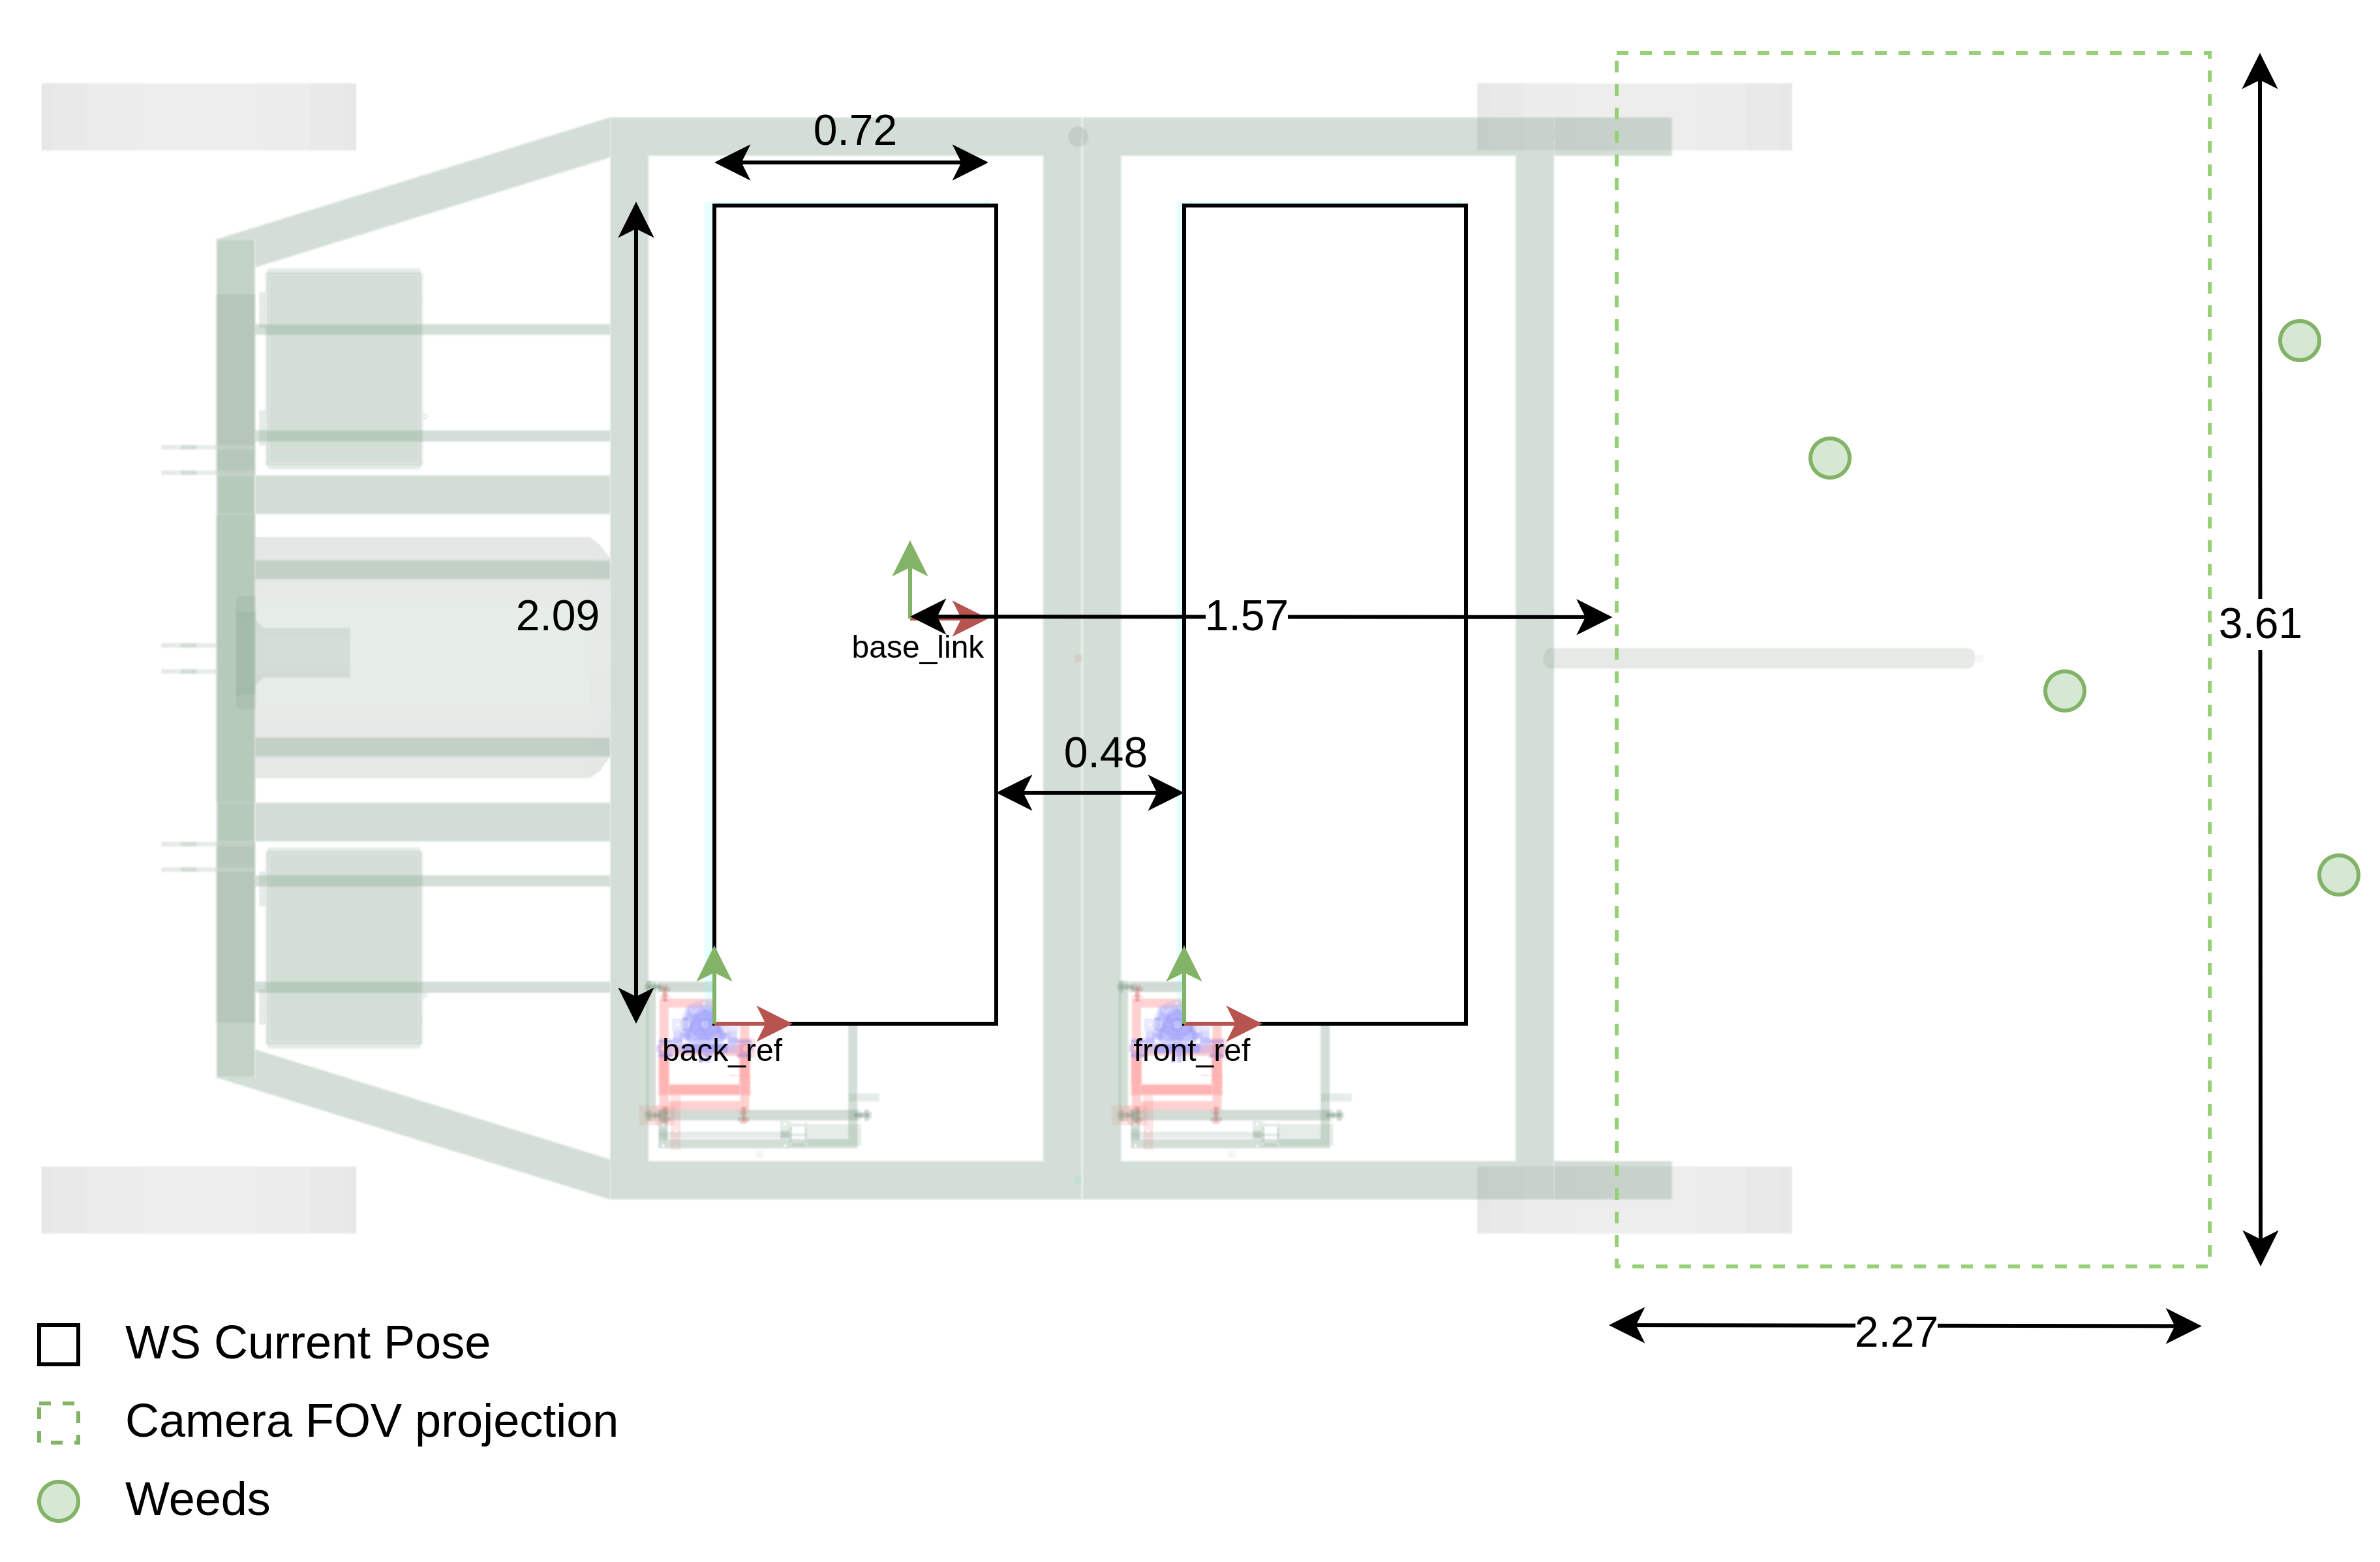
\includegraphics[width=\linewidth]{gfx/ch03/problem_layout.png}
    \caption{Problem Layout Dimentions}
    \label{fig:problem-layout.png}
\end{figure}

\section{Metrics}
Defining a good set of metrics is crucial to establish a solid basis for comparison between solutions and to easily identify the flaws of each method, thereby determining the best solution. To address this, we define two main categories. The first summarizes mission-level metrics such as the total idle and productive time of each tool, and the total time the robot spends moving or in a stationary state (defined by equations \ref{eq:total-mission-time} and \ref{eq:tool-usage-time}). The second category includes task-specific information, for example, task ID, status ('\textit{compleated}', '\textit{failed}', '\textit{out}'), number of stops, the tool that processed the task, and the idle and productive time of each tool at that specific stop. These metrics are displayed in a mission dashboard for easy visualization and comparison across missions using different worlds or algorithms (see \autoref{fig:mission-metrics} for the first category and \ref{fig:task-metrics} for the second one).

\begin{figure}[htb]
    \myfloatalign
    \subfloat[Mission Category Metrics]
    {\label{fig:mission-metrics}
        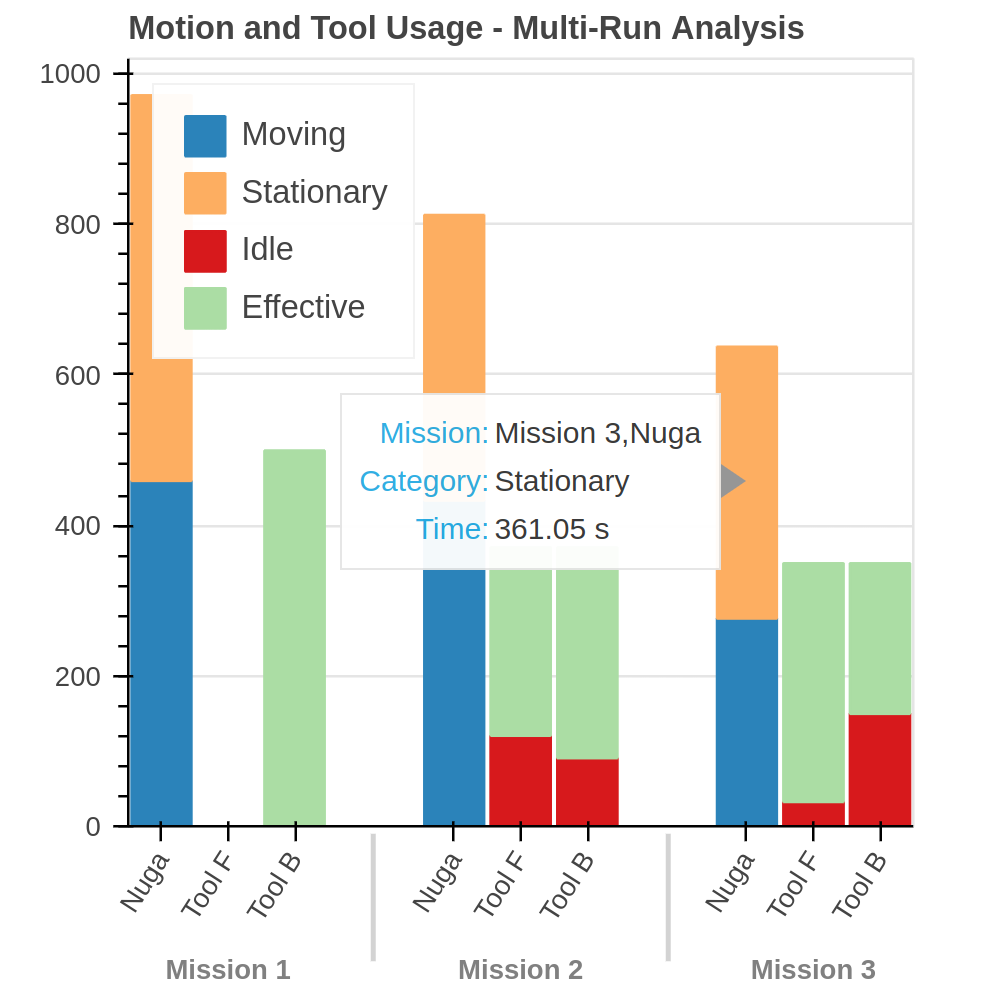
\includegraphics[width=.45\linewidth]{gfx/ch03/mission_metrics.png}} \quad
    \subfloat[Task Visualization]
    {\label{fig:task-metrics}%
        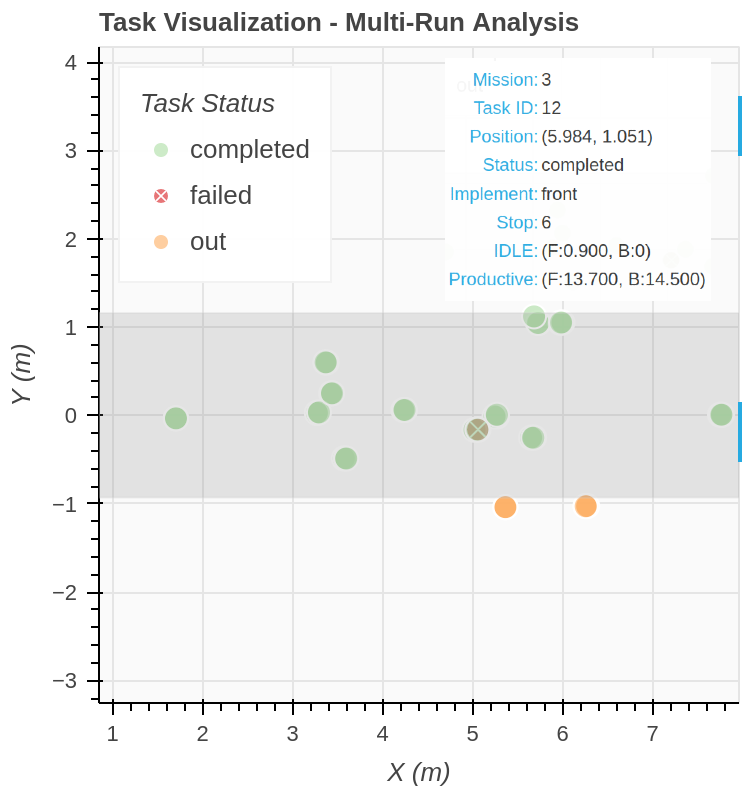
\includegraphics[width=.45\linewidth]{gfx/ch03/task_metrics.png}} \\
    \caption{Mission Dashboard}\label{fig:mission-dashboard}
\end{figure}


\paragraph{\autoref{fig:mission-metrics}} Showcases a bar graph comparing different missions. Each mission includes the robot's moving and stationary time, as well as the idle and productive time of the onboard implement tools. A hover feature displays the value of each category.

\paragraph{\autoref{fig:task-metrics}} Displays a 2D grid of the removed tasks' positions during the mission, along with their corresponding metadata. Hovering over a task reveals its details, and tasks can be filtered by mission.

\begin{equation}
    t_{mission} = t_{moving} + t_{stationary}
\label{eq:total-mission-time}
\end{equation}

\begin{equation}
    t_{tool\_operation} = t_{idle} + t_{productive}
\label{eq:tool-usage-time}
\end{equation}


\section{Heuristics}
Heuristic solutions are commonly employed when the solution space of an optimization problem is too large to explore exhaustively, making an exact optimal solution computationally infeasible. They are also useful in time-sensitive scenarios, such as online implementations, where sacrificing optimality for efficiency is often justified.

In our work, we developed a heuristic algorithm to serve as a baseline solution, this provides a meaningful reference point to assess the performance and potential improvements offered by other algorithms. The algorithm' description is detailed in \ref{alg:heuristic}, with an illustrative example in \autoref{fig:heuristic-steps}.

\begin{algorithm}
    \caption{Heuristic}
    \begin{algorithmic}[1]
        \STATE Get the position of the closest weed from the current robot position.  
        \STATE Project the tools' \ac{WS} forward (in the future), aligning the trailing edge of the last \ac{WS} with the closest weed's position plus a small clearance (e.g., 10 cm).  
        \STATE Allocate weeds to each tool if they fall within its projected \ac{WS}.
        \STATE Move the robot until the tools' \ac{WS} are aligned with their projections, then execute the extractions for tools with assigned weeds.  
        \STATE Repeat the process until mission has ended.  
    \end{algorithmic}
    \label{alg:heuristic}
\end{algorithm}

\begin{figure}[htb]
    \myfloatalign
    \subfloat[S1.Closest task, S2.WS projection]
    {\label{fig:heuristic-s1-s2}
        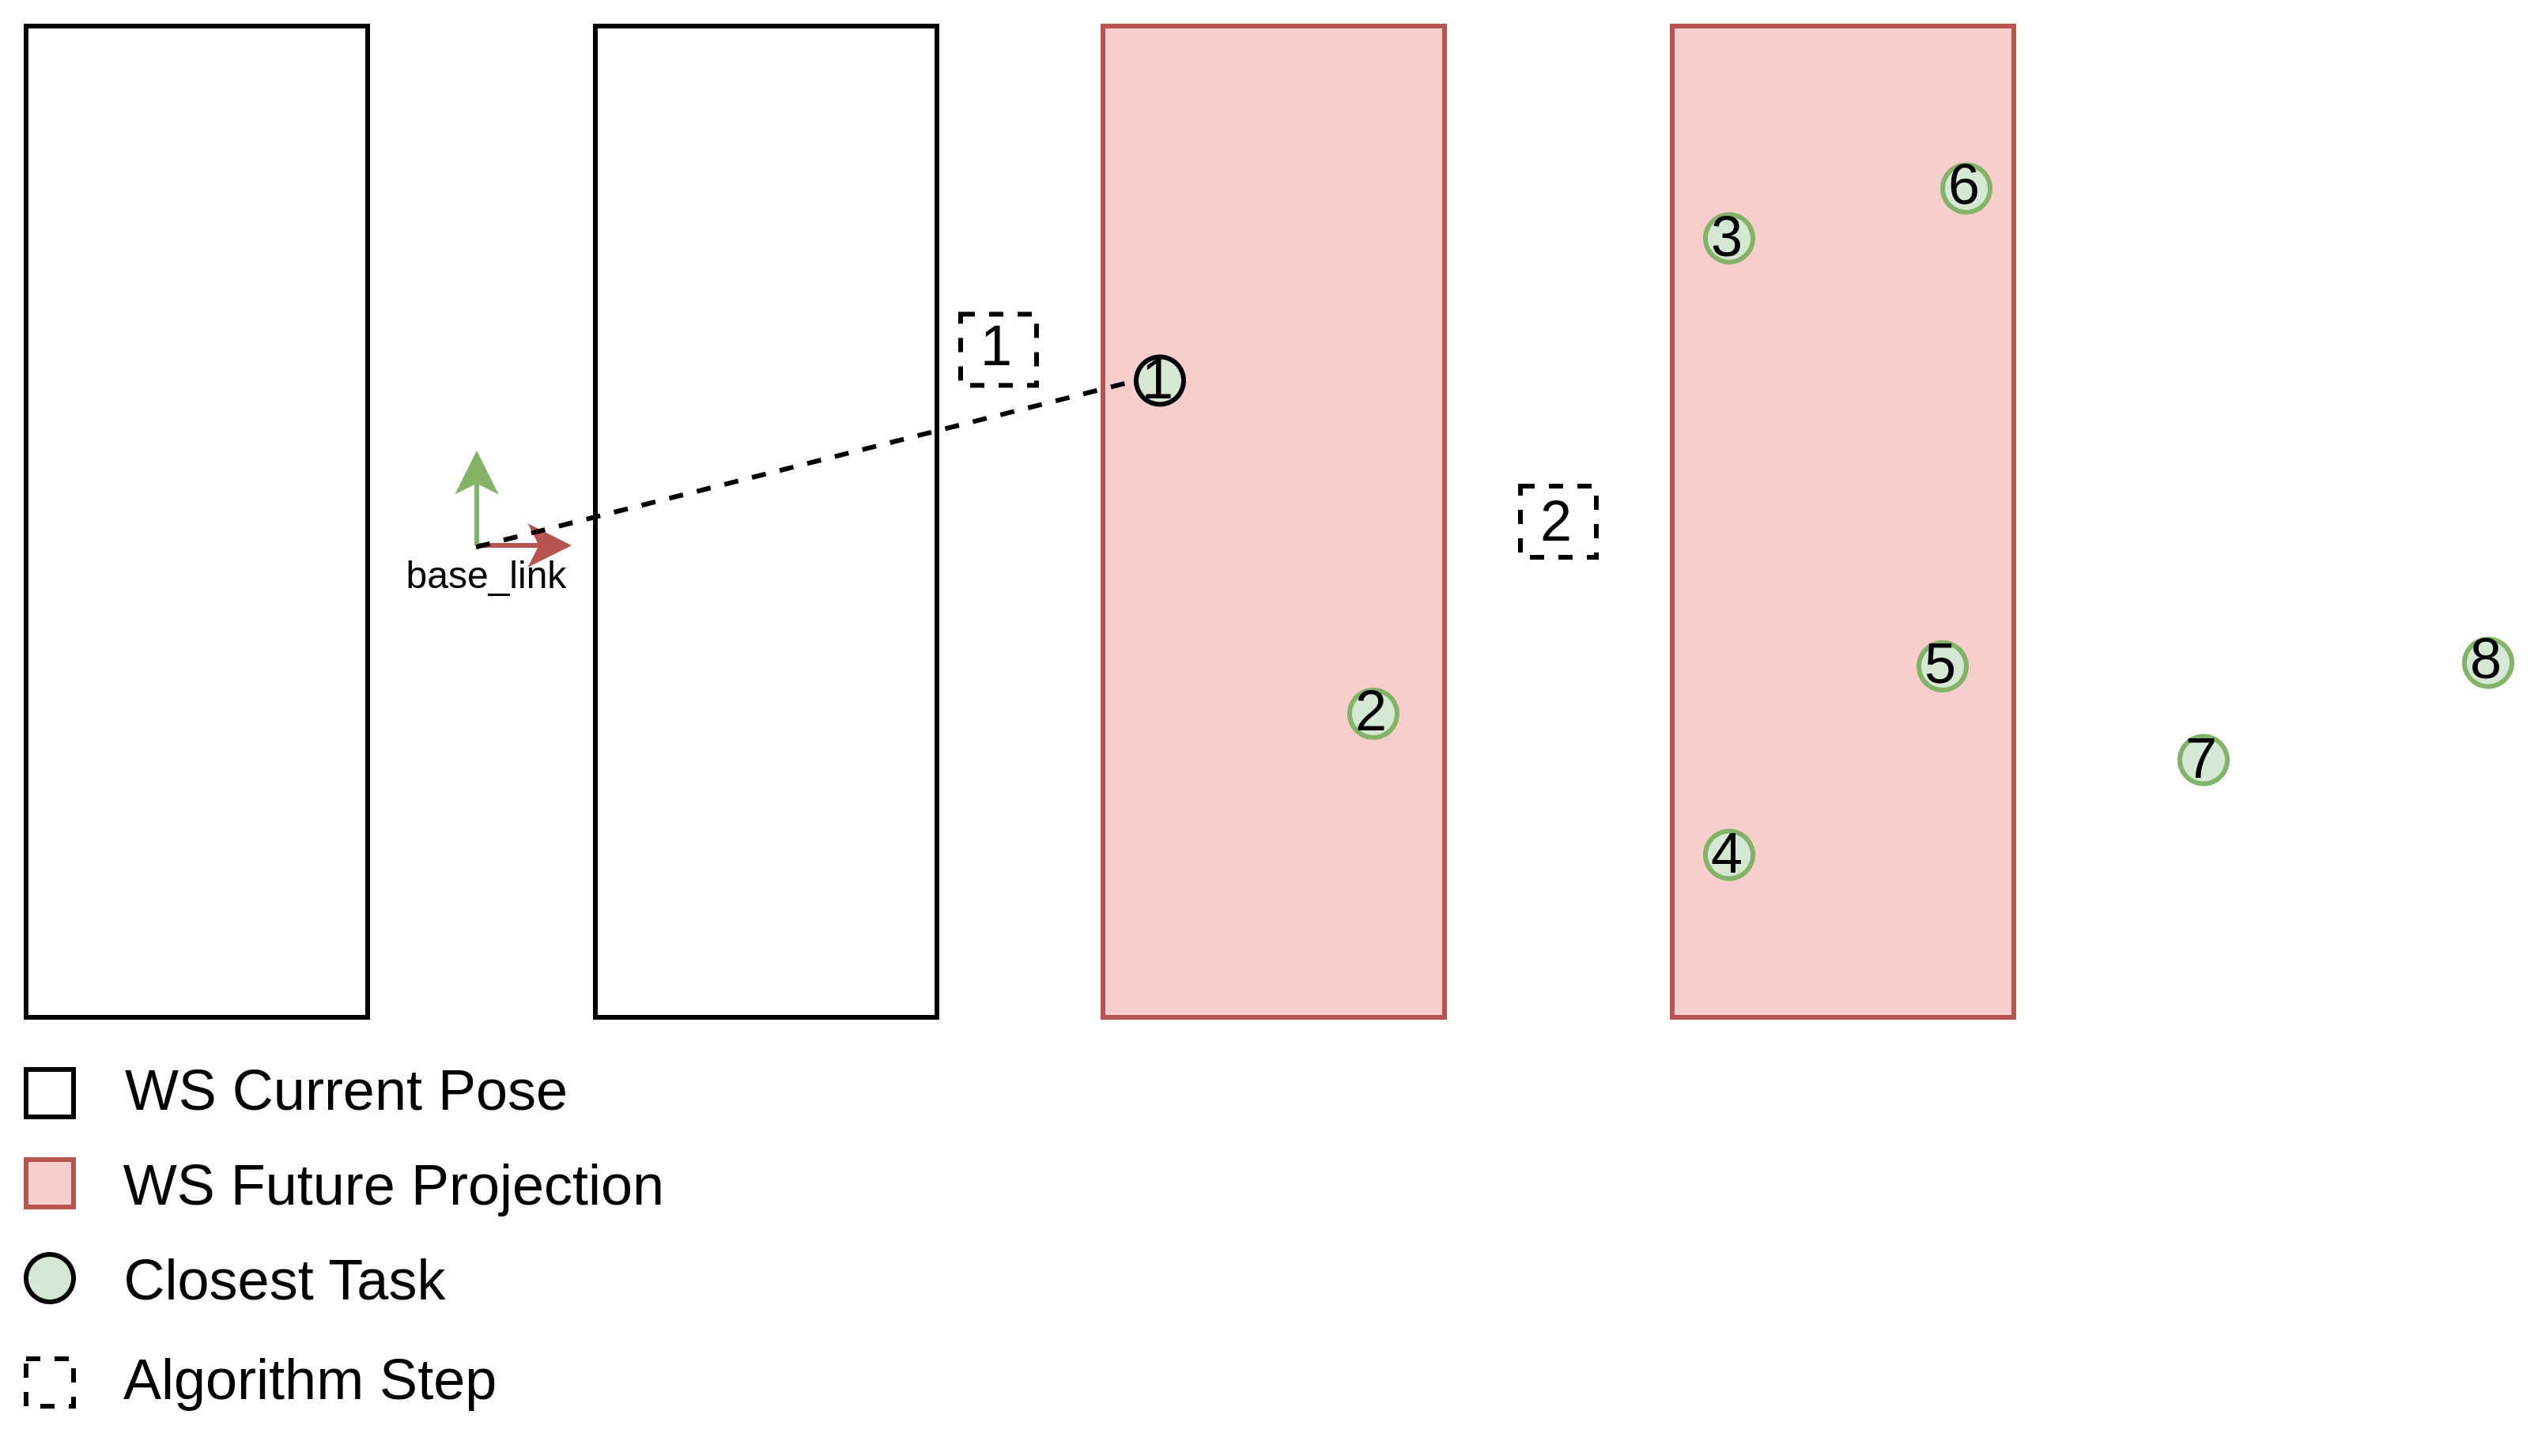
\includegraphics[width=.50\linewidth]{gfx/ch03/heuristic_s1_s2.png}} \quad
    \subfloat[S3.Task Allocation]
    {\label{fig:heuristic-s3}%
        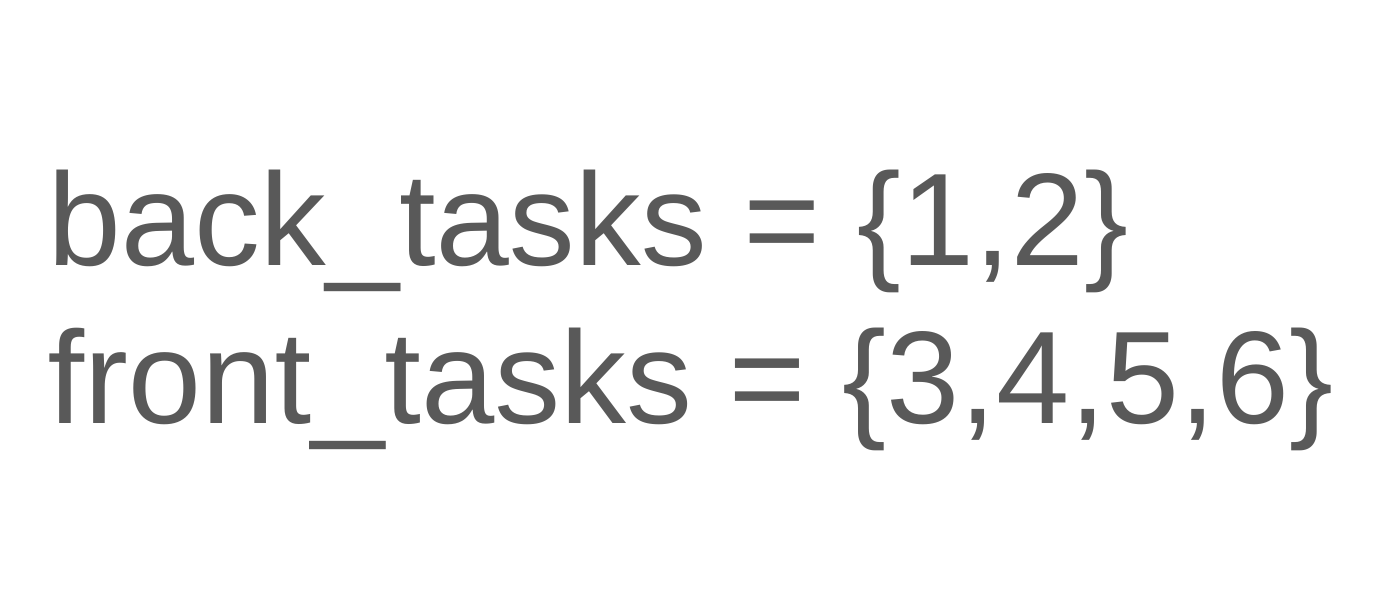
\includegraphics[width=.40\linewidth]{gfx/ch03/heuristic_s3.png}} \\
    \subfloat[S4.Moving until aligned and extraction]
    {\label{fig:heuristic-s4}
        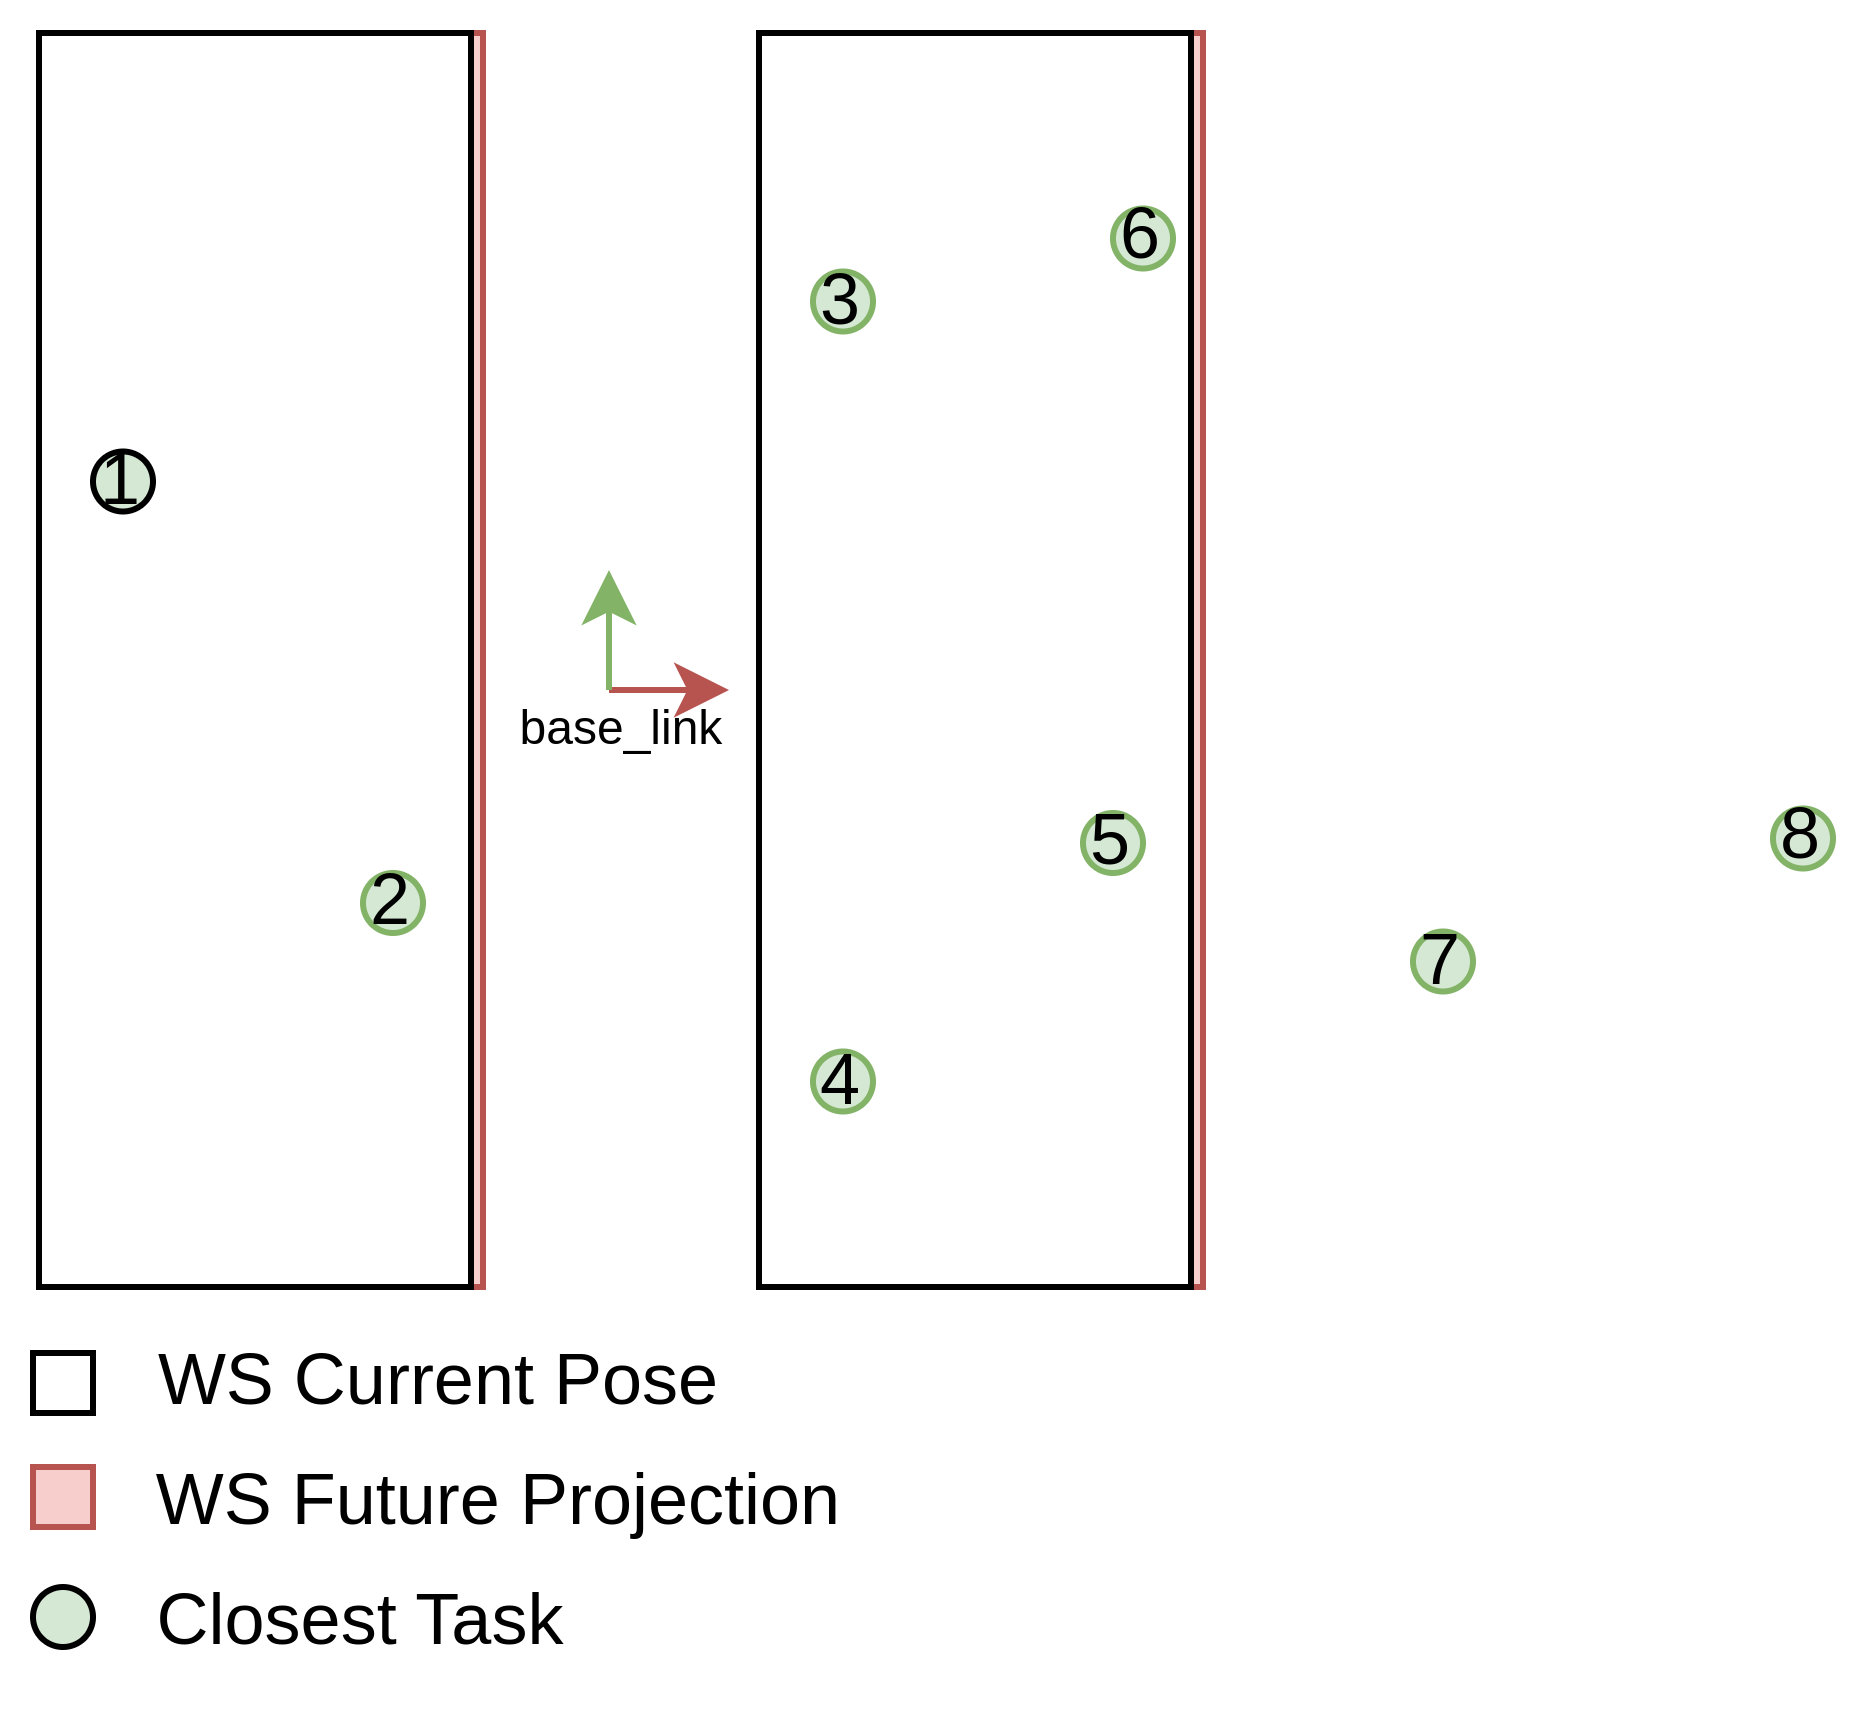
\includegraphics[width=.40\linewidth]{gfx/ch03/heuristic_s4.png}} \quad
    \subfloat[S5.Repeat]
    {\label{fig:heuristic-s5}%
        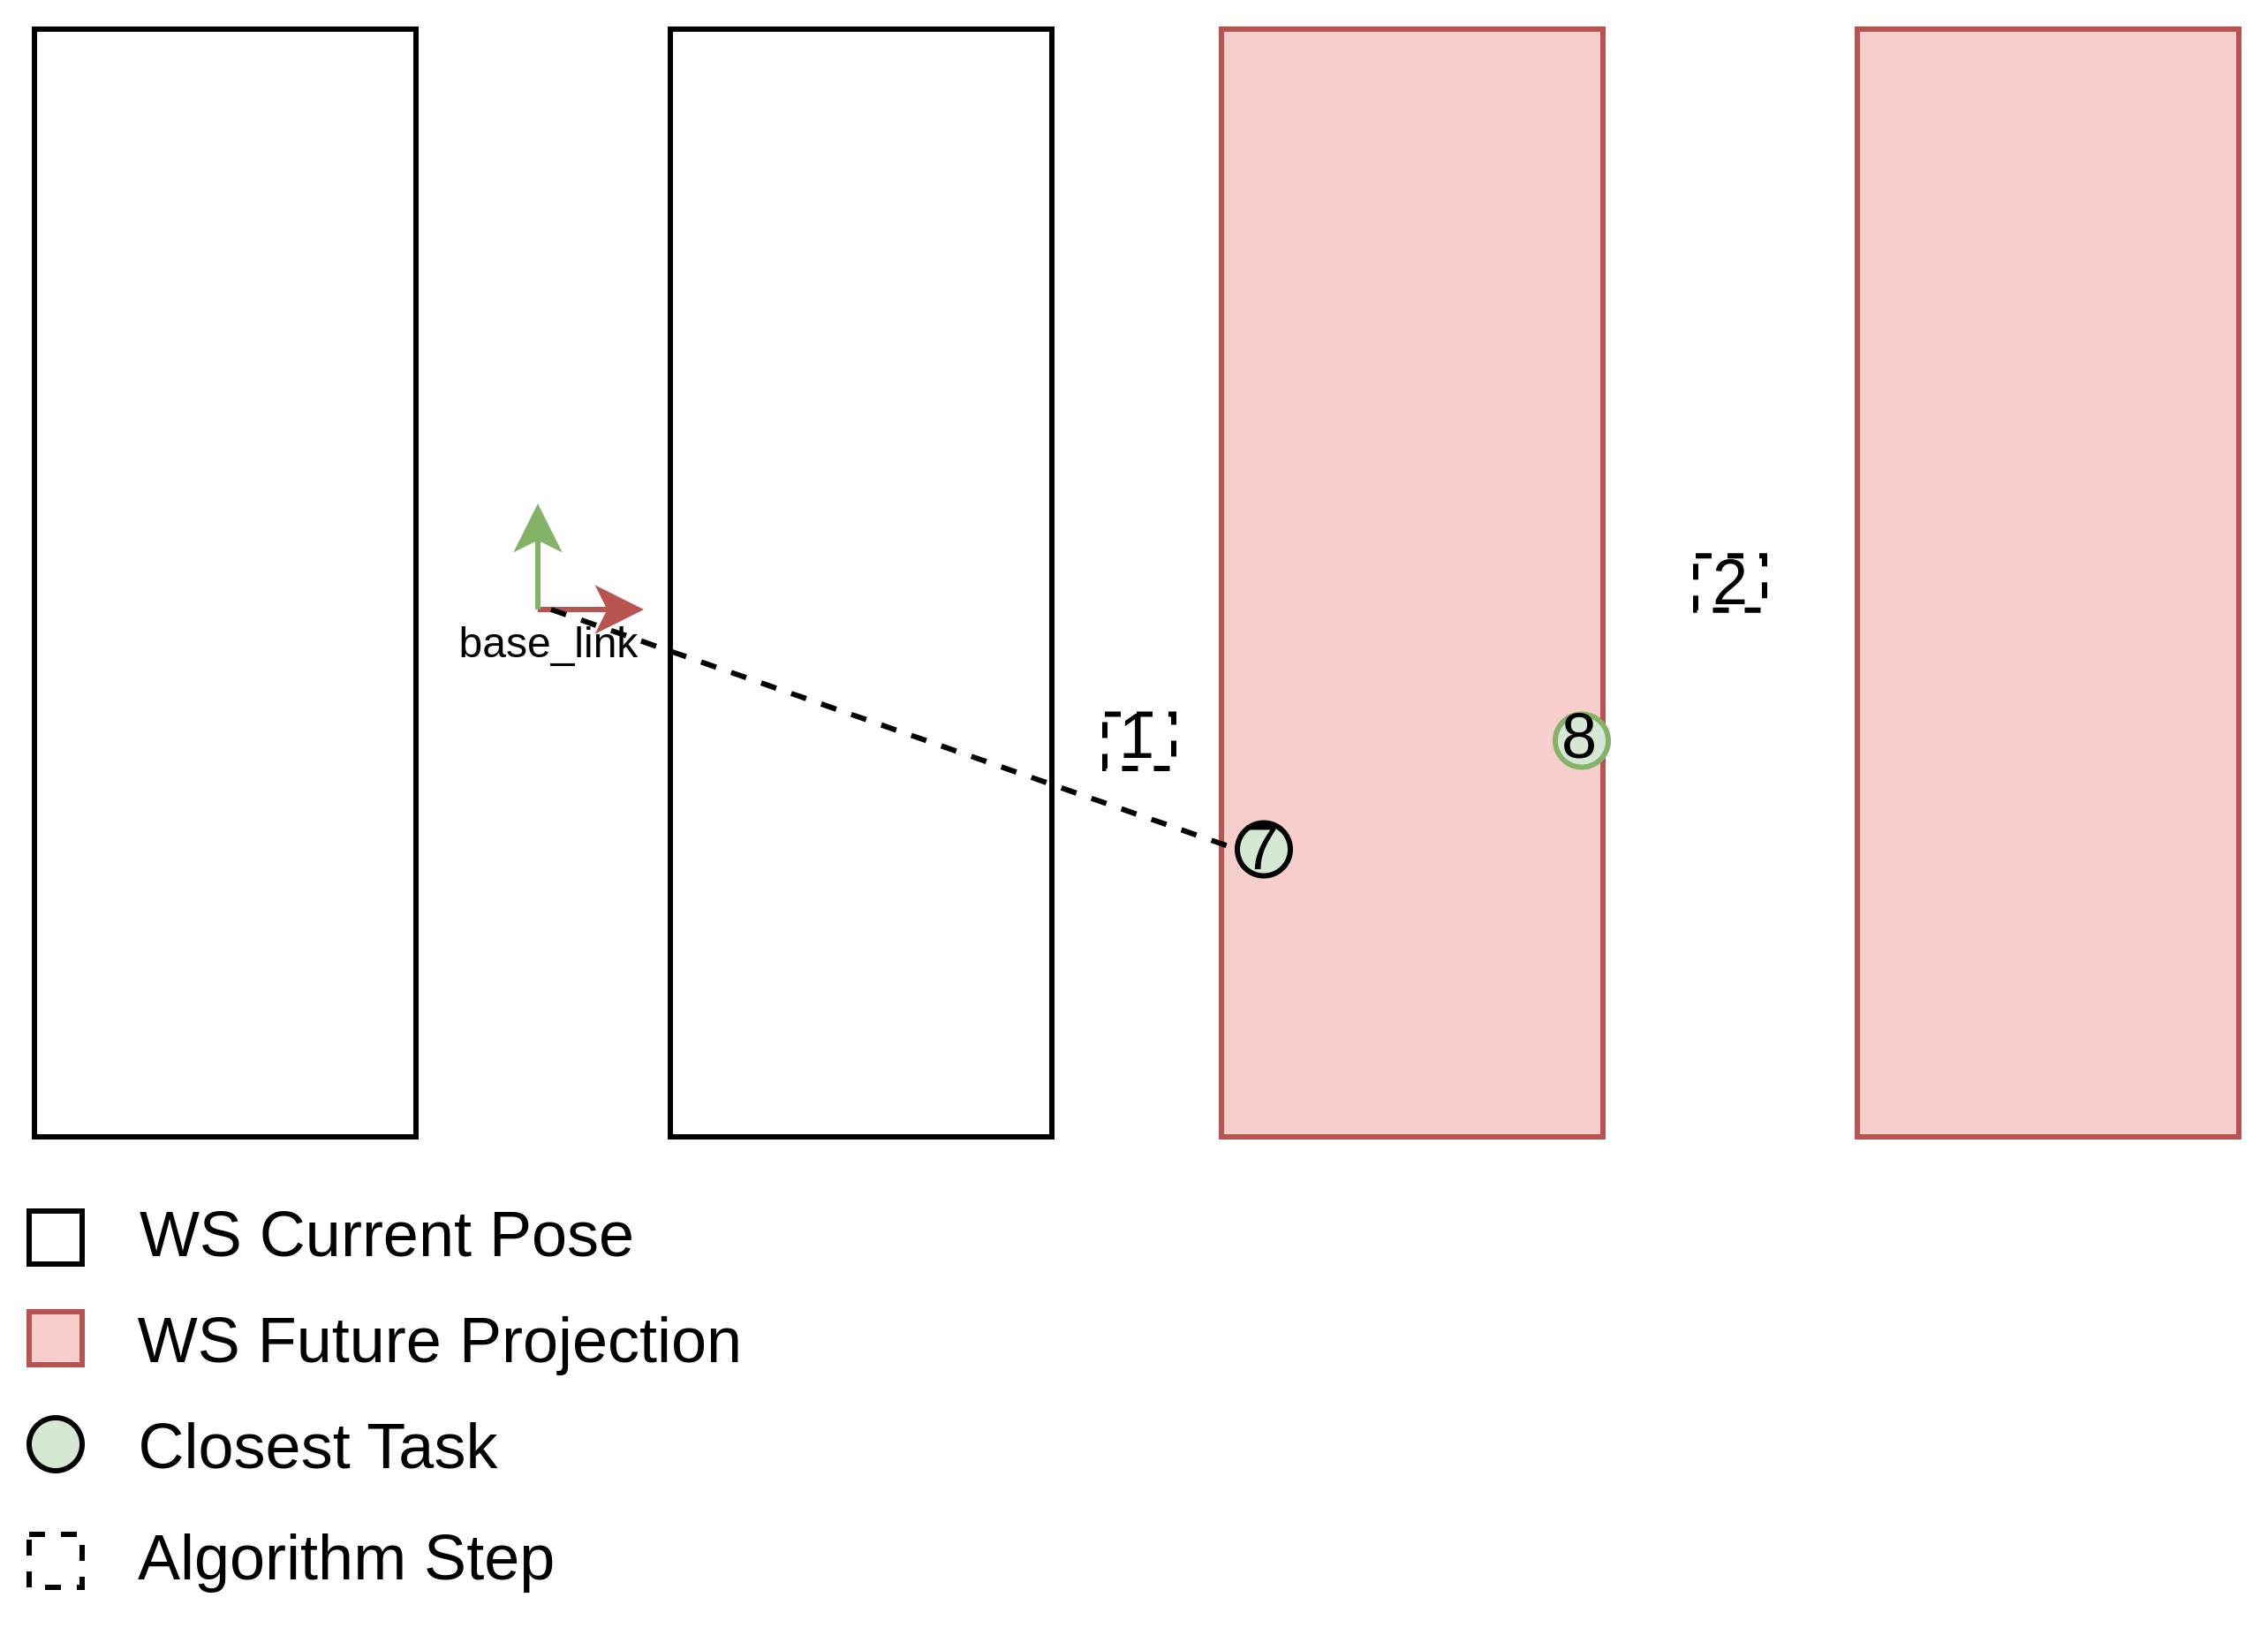
\includegraphics[width=.50\linewidth]{gfx/ch03/heuristic_s5.png}} \\
    \caption{Heuristic Algorithm}\label{fig:heuristic-steps}
\end{figure}

This approach offers a simple implementation and fast computation solution, making it well-suited for online applications. However, its heuristic nature leads to suboptimal solutions, as it does not account for minimizing idle time. In \autoref{fig:heuristics-suboptimal} we exemplify the algorithm' suboptimality for a particular case, contrasting with a better solution to support our analysis.

\paragraph{\autoref{fig:heuristic-suboptimal-stops}} Showcases the two stops required to remove eight weed' detections, with the first stop allocating four tasks to the back tool and the second stop allocating two tasks to the front tool.

\paragraph{\autoref{fig:heuristic-suboptimal-time}} Illustrates the idle and productive time for the given solution. Blue represents the robot’s repositioning time, red indicates the idle time of the respective tool, and white the productive time. The first stop shows a significant idle time for the front tool (90 seconds, equivalent to two tasks), caused by the tool waiting for the back tool to finish before proceeding to the next stop. The second stop shows a similar situation, where idle time arises from the only feasible option at that point: removing tasks 5 and 6 with the back tool.

\begin{figure}[htb]
    \myfloatalign
    \subfloat[Two stops required]
    {\label{fig:heuristic-suboptimal-stops}
        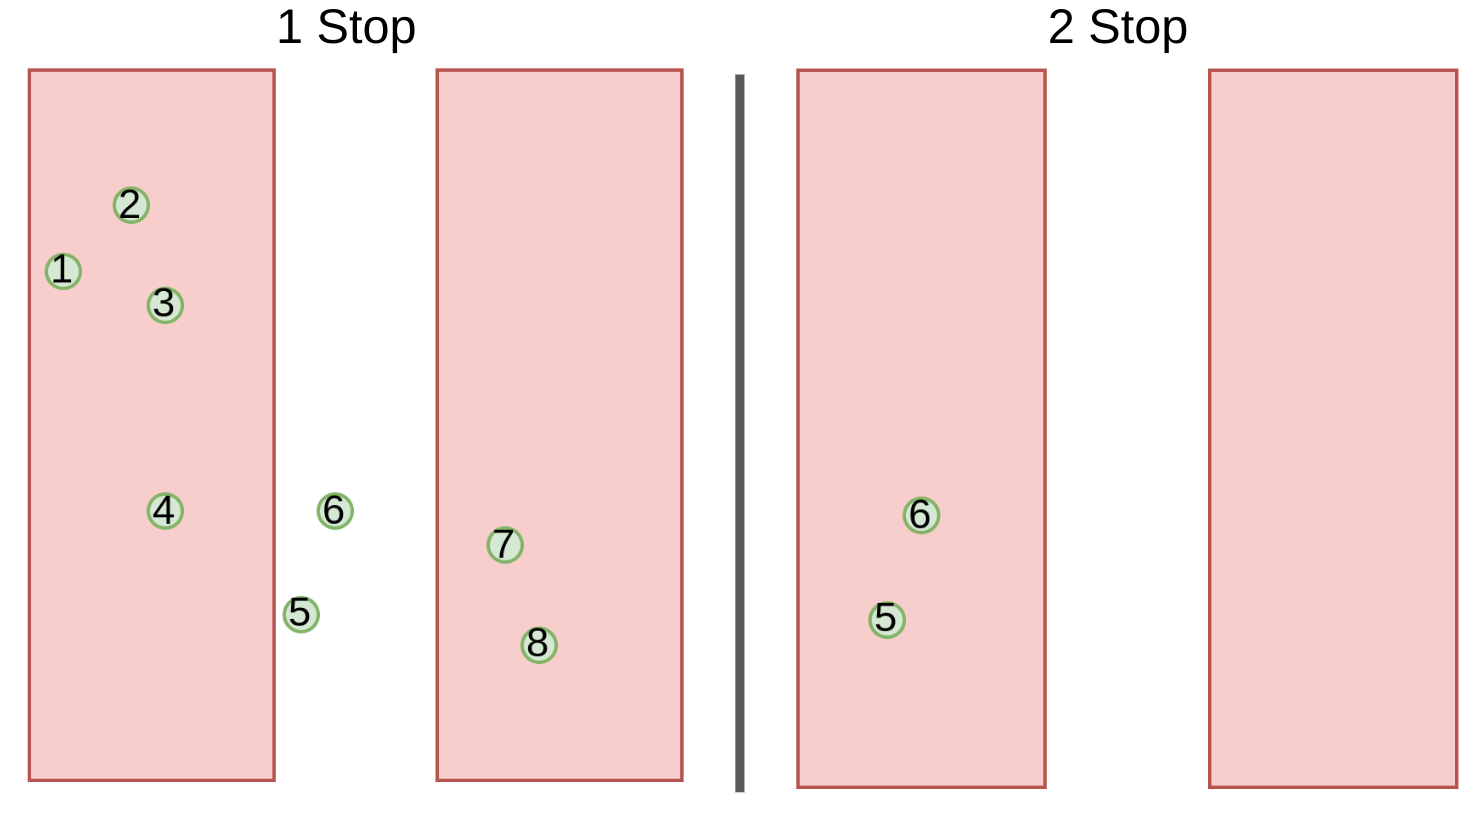
\includegraphics[width=0.6\linewidth]{gfx/ch03/heuristic_suboptimal_stops.png}}

    \subfloat[Idle and productive time of each tool]
    {\label{fig:heuristic-suboptimal-time}
        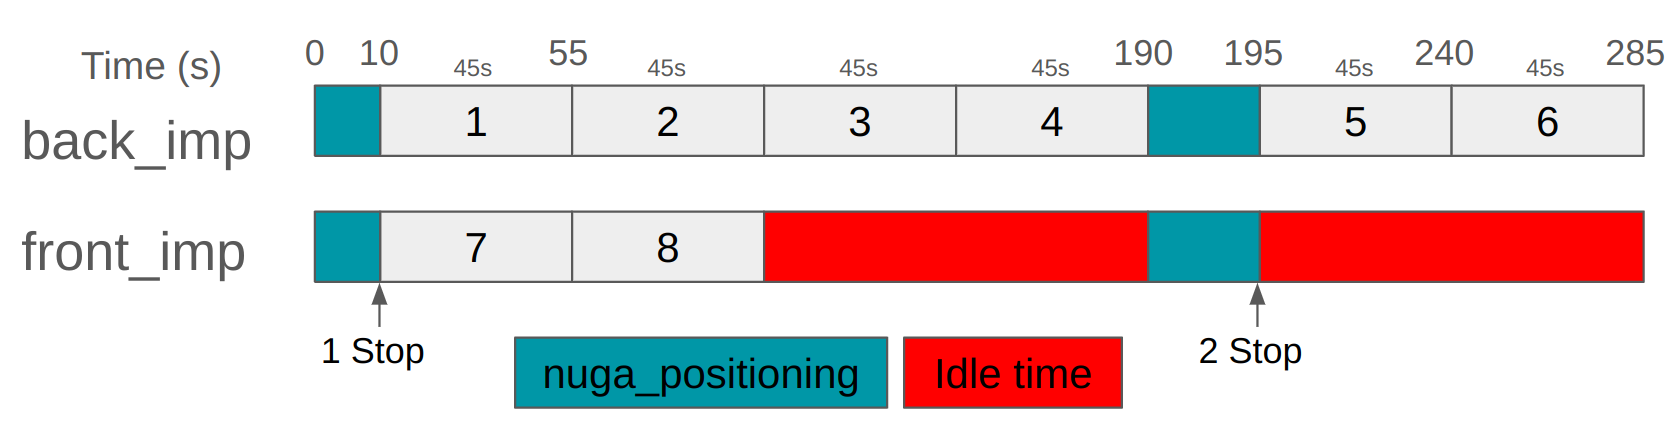
\includegraphics[width=0.9\linewidth]{gfx/ch03/heuristic_suboptimal_time.png}}

    \caption{Suboptimal solution computed using Heuristic}
    \label{fig:heuristics-suboptimal}
\end{figure}

An alternative solution for the same scenario (this time aimed at reducing idle time) is illustrated in \autoref{fig:heuristics-optimal}. In this case, the solution requires three stops: first stop assigns tasks 1 to back tool and task 5 to the front, the second stop processes tasks 2 and 6, and finally the third stop is used to remove tasks 3, 4, 7, and 8. As shown in \autoref{fig:heuristic-optimal-time}, the balanced task allocation between tools eliminates idle time and reduces the total mission duration compared to the previous solution.

This demostrates the heuristic's suboptimality, as it fails to minimize idle time and does not consider the possibility of stopping at a location that allows for a more efficient task allocation. The heuristic algorithm is limited to the closest weed detection, which may not always be the best option. In the following sections, we will explore more sofisticated algorithms that can overcome these limitations and provide better solutions. 

\begin{figure}[hbt]
    \myfloatalign
    \subfloat[Three stops required]
    {\label{fig:heuristic-optimal-stops}
        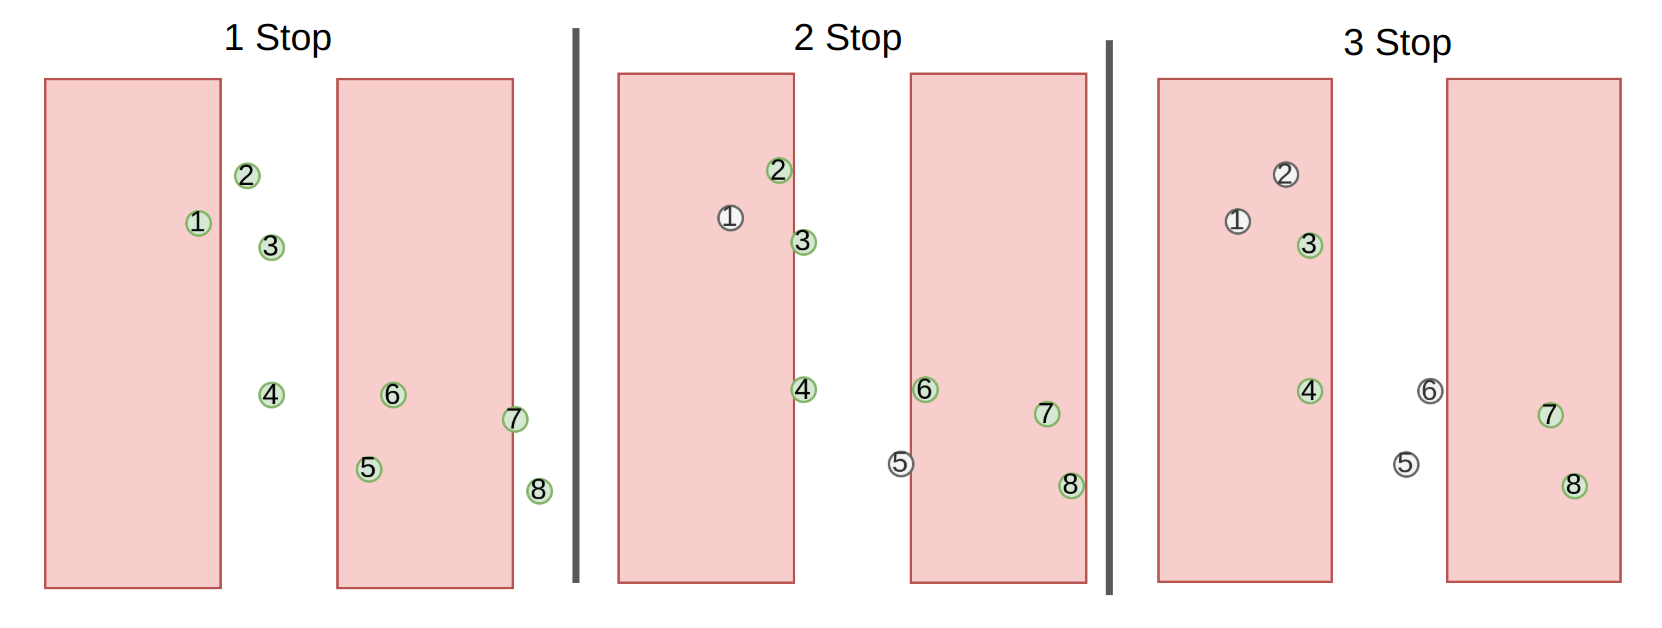
\includegraphics[width=0.6\linewidth]{gfx/ch03/heuristic_optimal_stops.png}}

    \subfloat[Idle and productive time of each tool]
    {\label{fig:heuristic-optimal-time}
        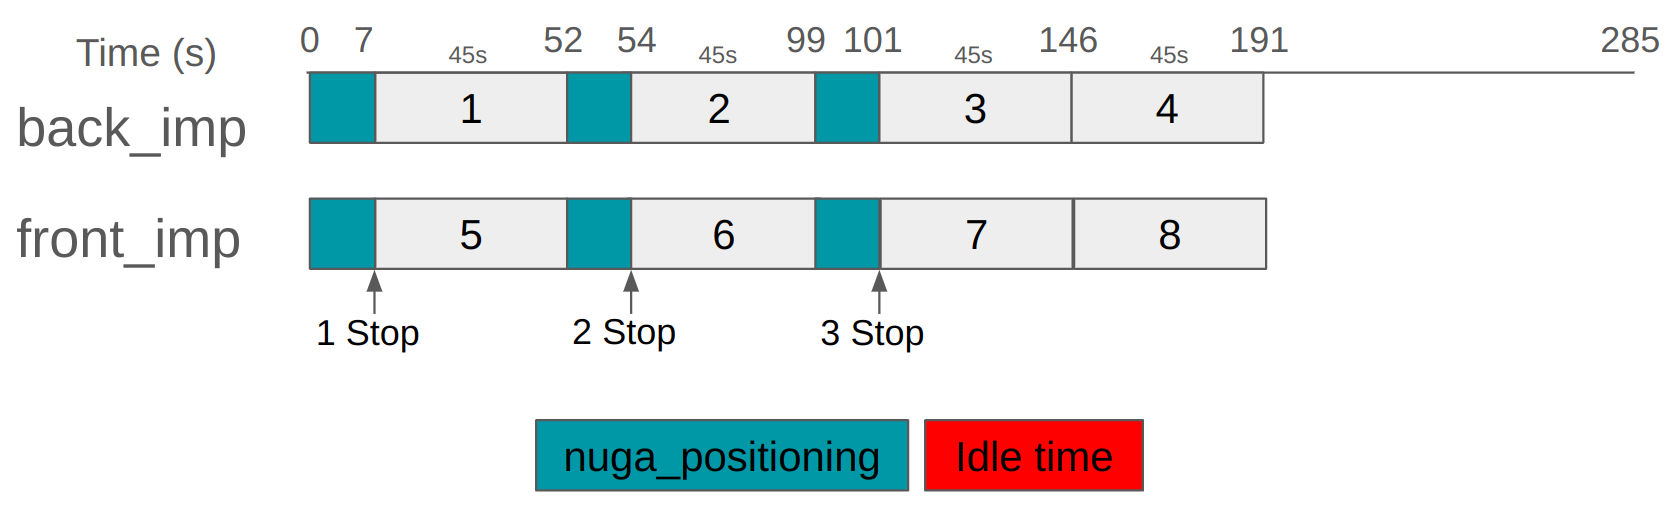
\includegraphics[width=0.9\linewidth]{gfx/ch03/heuristic_optimal_time.png}}

    \caption{Optimal solution}
    \label{fig:heuristics-optimal}
\end{figure}

\section{Graph Search}
Graph Search are a type of algorithms widely used in graph theory to systematically explore or traverse a graph. They are commonly used to find the shortest path between nodes, identify connected components, or solve various optimization problems. Graph search algorithms can be broadly categorized into two main types: uninformed and informed search algorithms.

Uninformed search algorithms do not have any additional information about the problem domain and explore the graph blindly. Examples include \ac{DFS} and \ac{BFS}. These algorithms are typically used for tasks like finding connected components or traversing all nodes in a graph.
Informed search algorithms, on the other hand, use heuristics or additional information to guide the search process. They are often more efficient than uninformed algorithms for specific problems. Examples include A* search and Dijkstra's algorithm, which are commonly used for finding the shortest path in weighted graphs.

In our context, we exploit the advantages of graph-based algorithms by modeling the problem as such. Nodes represent potential stop locations, where two types of actions are possible: moving to another stop (a \textit{stop node}) or performing weed removal at that location (an \textit{action node}). Edge weights are defined as follows: edges between two \textit{stop nodes} represent \textit{travel cost}, computed using the distance between stops and the robot’s velocity or a unitary value as a placeholder. Edges connecting a \textit{stop node} to an \textit{action node} represent \textit{task execution cost}, and it is calculated based on the idle time (if any) of removing the indicated weeds with the assigned tools.

\begin{figure}[hbt]
    \centering
    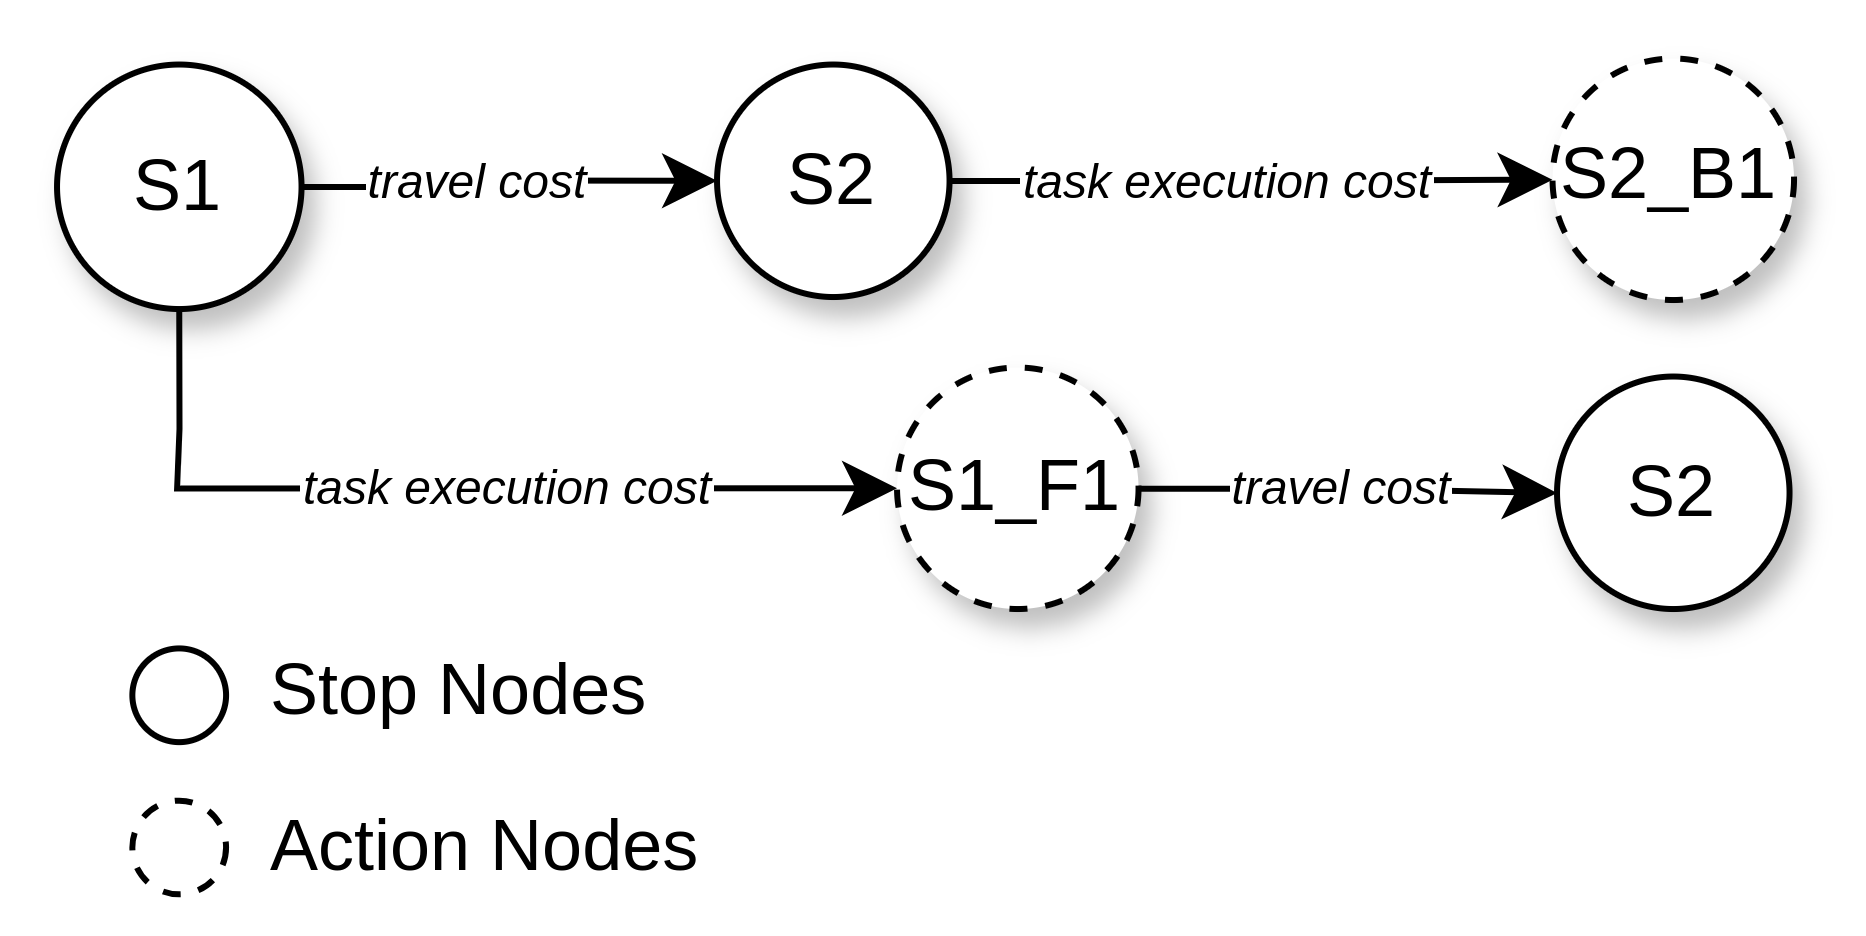
\includegraphics[width=0.8\linewidth]{gfx/ch03/graph_search_nodes.png}
    \caption{Node types and cost representation}
    \label{fig:graph-search-nodes}
\end{figure}

\paragraph{\autoref{fig:graph-search-nodes}} Illustrates the convention used to represent the graph. \texttt{S1} denotes stop number 1, while \texttt{F} or \texttt{B} indicate whether the front or back tool is assigned to remove the weed, followed by the weed ID to be processed. In this example, the task execution cost between \texttt{S1} and \texttt{S1\_F1} would be 45s, as the back tool must wait for the front tool to process 1 plant. The same logic applies to the cost between \texttt{S2} and \texttt{S2\_B1} but for the front tool.

The graph search implementation solution follows the next pipeline:
\begin{enumerate}
    \item Compute \textbf{candidate stops} based on the robot's current position and weed detections. Candidate stops are the locations where an important event ocurs, such as a weed entering or exiting the workspace of a tool.
    \item \textbf{Associate} reachable weeds with candidate stops. This allows the algorithm to determine which weeds can be removed at each stop.
    \item Create a \textbf{graph representation} of the problem using \ac{DFS} algorithm and the convention described in \autoref{fig:graph-search-nodes}. The graph is built by connecting \textit{stop nodes} and \textit{action nodes} using appropriate edge costs, taking into account the predefined associations between stops and tasks.
    \item Get the \textbf{shortest path} in the graph from the root (first stop) to the final node (last stop) using Dijkstra's algorithm.
    \item \textbf{Decode solution} and return the next optimal stop and task allocation as the algorithm's output.
\end{enumerate}

% TODO: Later I could add explanation of step 1 and 2 of the pipeline, candidate stops and association

To build and explore the graph, an implementation of the \ac{DFS} algorithm is used (see Algorithm \ref{alg:dfs}). The \texttt{get\_children\_nodes} method expands the graph by generating child nodes from a given parent node. If the parent node is a \textit{stop node}, it creates child nodes for all valid combinations of reachable tasks that can be processed at that stop. Each combination forms a new child node that reflects the state after removing those tasks (\textit{action node}). Additionally a 'trivial' \textit{stop node} is addded representing the decision to move to the next stop without removing any weeds. On the other hand, if the parent node is an \textit{action node}, this method creates a single \textit{stop node} representing the next stop. Each created edge is added to the graph with a weight based on the associated \textit{task execution cost} or \textit{travel cost}. \autoref{fig:building-graph} illustrates the graph expansion process, where the algorithm grows all possible combinations of tasks at each stop and generates the corresponding child nodes. 

We observe that from \texttt{S3} four possible states can be reached (three \textit{action nodes} and one \textit{stop node}), The transition \texttt{S3\_B1\_F2} achieves zero idle time by optimally balancing tasks between the front and back tools, whereas the other transitions result in higher idle times due to imbalanced assignments. It's important to note that the same stop can be reached through different paths, depending on the actions taken at previous stops. For instance, if task 1 has been removed earlier, it should no longer be considered in subsequent stops. This consideration is crucial when building the graph, as we must ensure that it is expanded only through valid and realistic transitions that reflect feasible execution scenarios.

\begin{figure}[hbt]
    \centering
    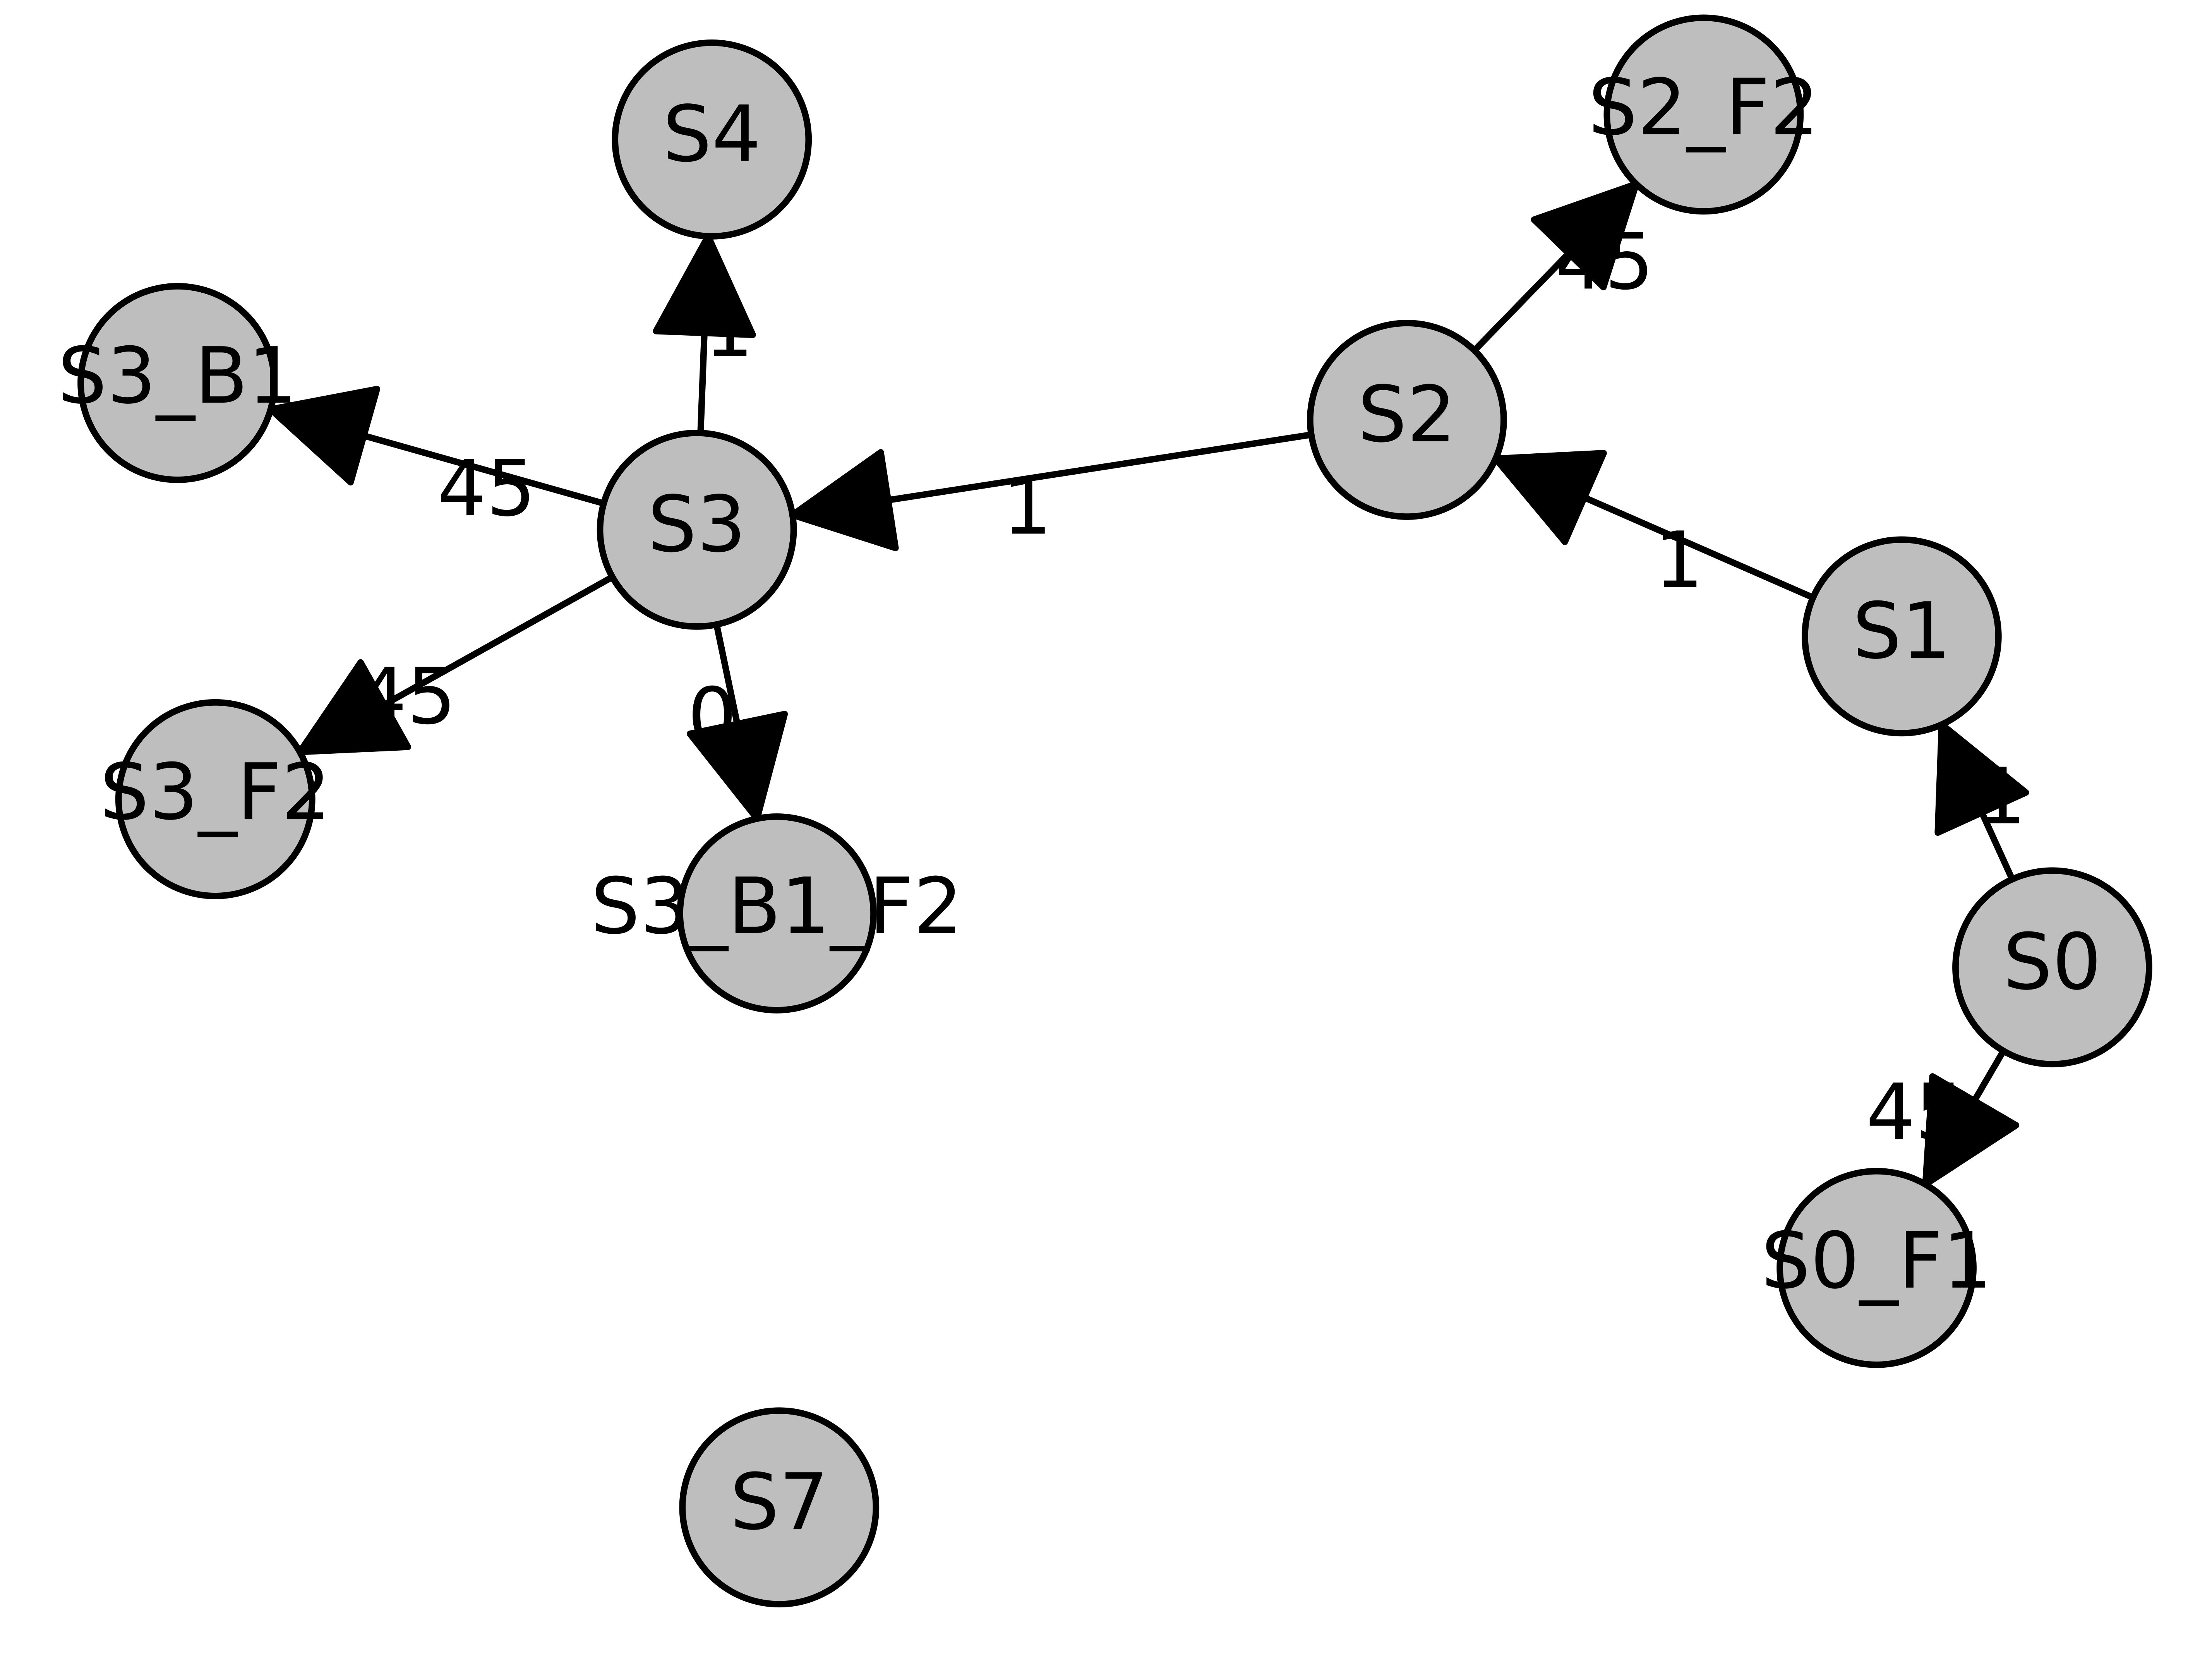
\includegraphics[width=0.7\linewidth]{gfx/ch03/building_graph.png}
    \caption{Graph expansion process}
    \label{fig:building-graph}
\end{figure}

Having the complete graph, and given its configuration as a weighted directed graph, we choose Dijkstra's algorithm to find the optimal path (see Algorihtm \ref{alg:dijkstra}). This algorithm efficiently explores the graph by maintaining a priority queue of nodes to be processed, ensuring that the node with the lowest cost is always explored first. The algorithm continues until it reaches the final node, which represents the optimal solution. The path is then traced back from the final node to the root, revealing the sequence of stops and actions that lead to the optimal solution.

\begin{figure}[htb]
    \myfloatalign
    \subfloat[Path with lowest cost]
    {\label{fig:graph-solution}
        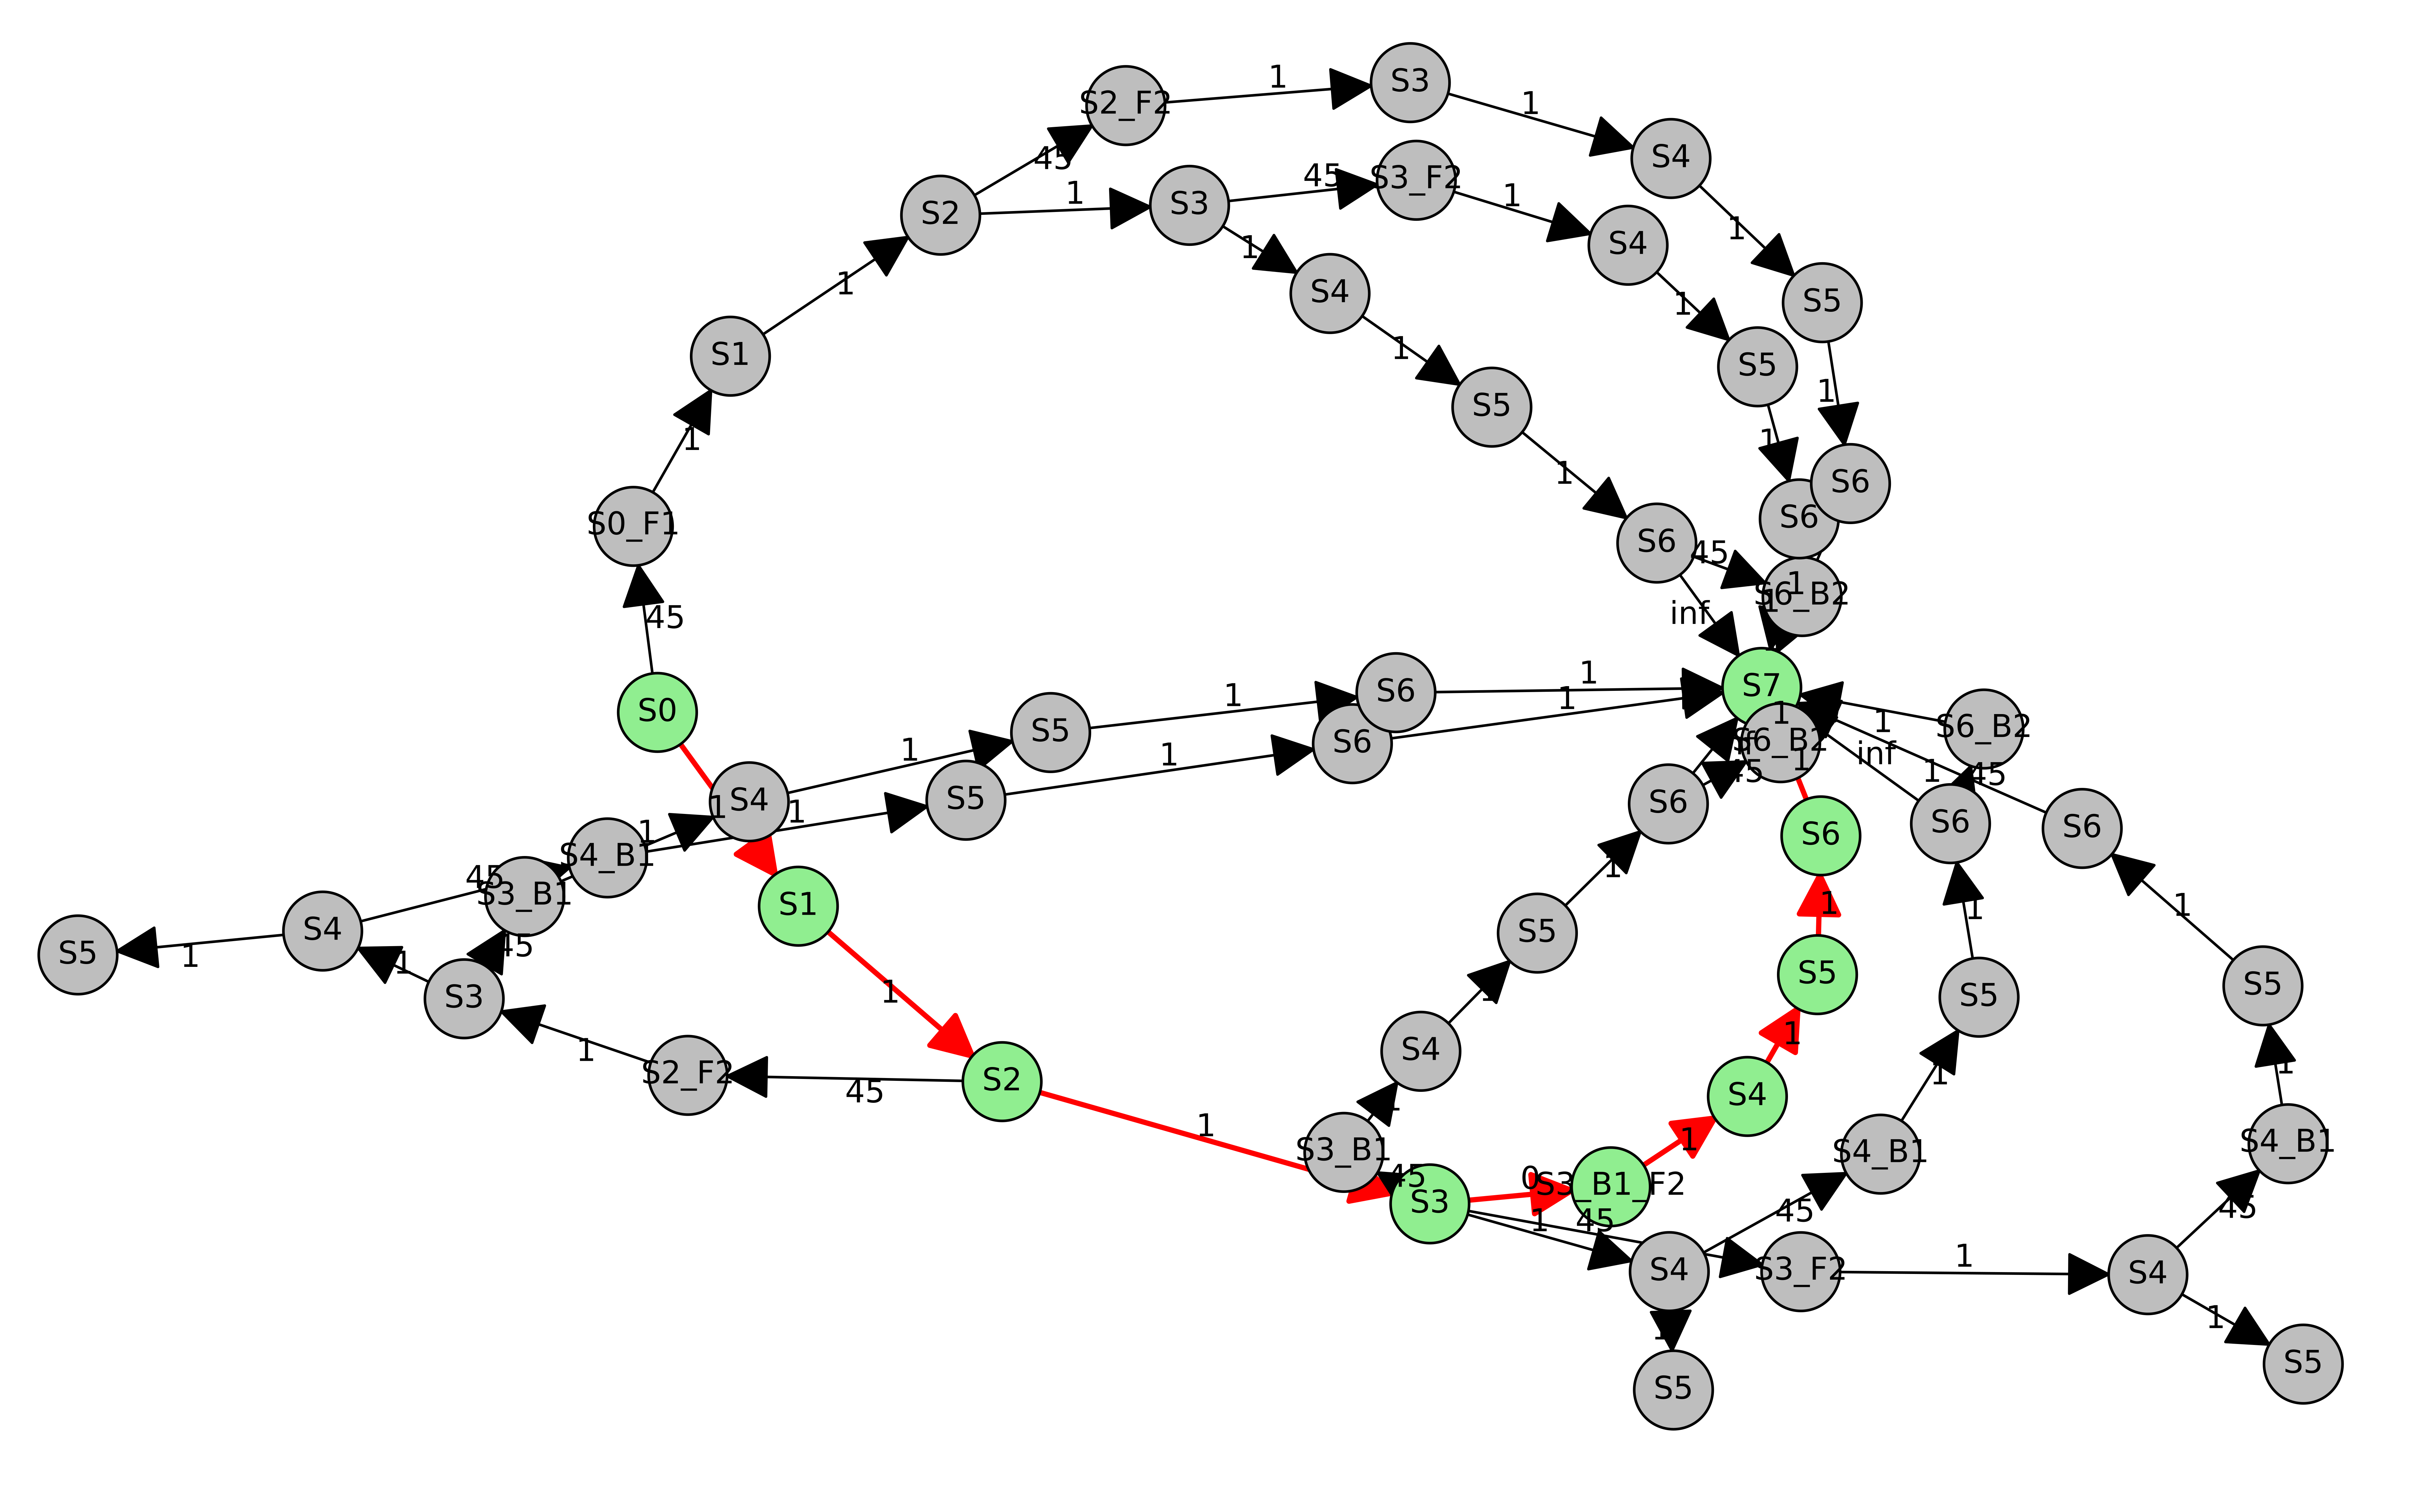
\includegraphics[width=.45\linewidth]{gfx/ch03/graph_solution.png}} \quad
    \subfloat[Task Planning Visualization]
    {\label{fig:scenario-2-tasks}%
        \includegraphics[width=.45\linewidth]{gfx/ch03/scenario_2_tasks.png}} \\
    \caption{Graph Search Solution}\label{fig:graph-search-solution}
\end{figure}

An optimal solution obtained by the graph search algorithm in a scenario with two detected weeds is illustrated in \autoref{fig:graph-solution}. The highlighted branch corresponds to the optimal path found by the algorithm. For the given two weeds, the graph contained 54 nodes, and the computation time was 0.001 seconds. A visual representation of the solution is shown in \autoref{fig:scenario-2-tasks}, including the current robot pose, projected workspaces in red, candidate stops in blue, and weeds in green.

% How we avoid the algorithm chossing trivial solutions where no weeds are removed?
One remaining issue to address is preventing the algorithm from returning trivial solutions in which either no weeds are removed or not all of them are. To tackle this, each node keeps track of the tasks completed so far. If, at the second-to-last node, there are still tasks left to remove, we assign a penalty cost to the edge leading to the final node. This encourages the algorithm to prioritize removing as many weeds as possible before proceeding to the last stop.

Our graph search solution performs well in terms of computation time, for a low to medium density of weeds. However, as the number of weeds increases, the graph size grows exponentially, leading to longer computation times. \autoref{fig:graphsearch-performance} showcases the graph size and computation time for different number of weeds (see plot in red). The graph size is defined as the number of nodes in the graph, while the computation time is the time required to build and find the optimal path in the graph.

\begin{figure}[htb]
    \myfloatalign
    \subfloat[Graph size vs. number of weeds]
    {\label{fig:graphsearch-graph-size}%
        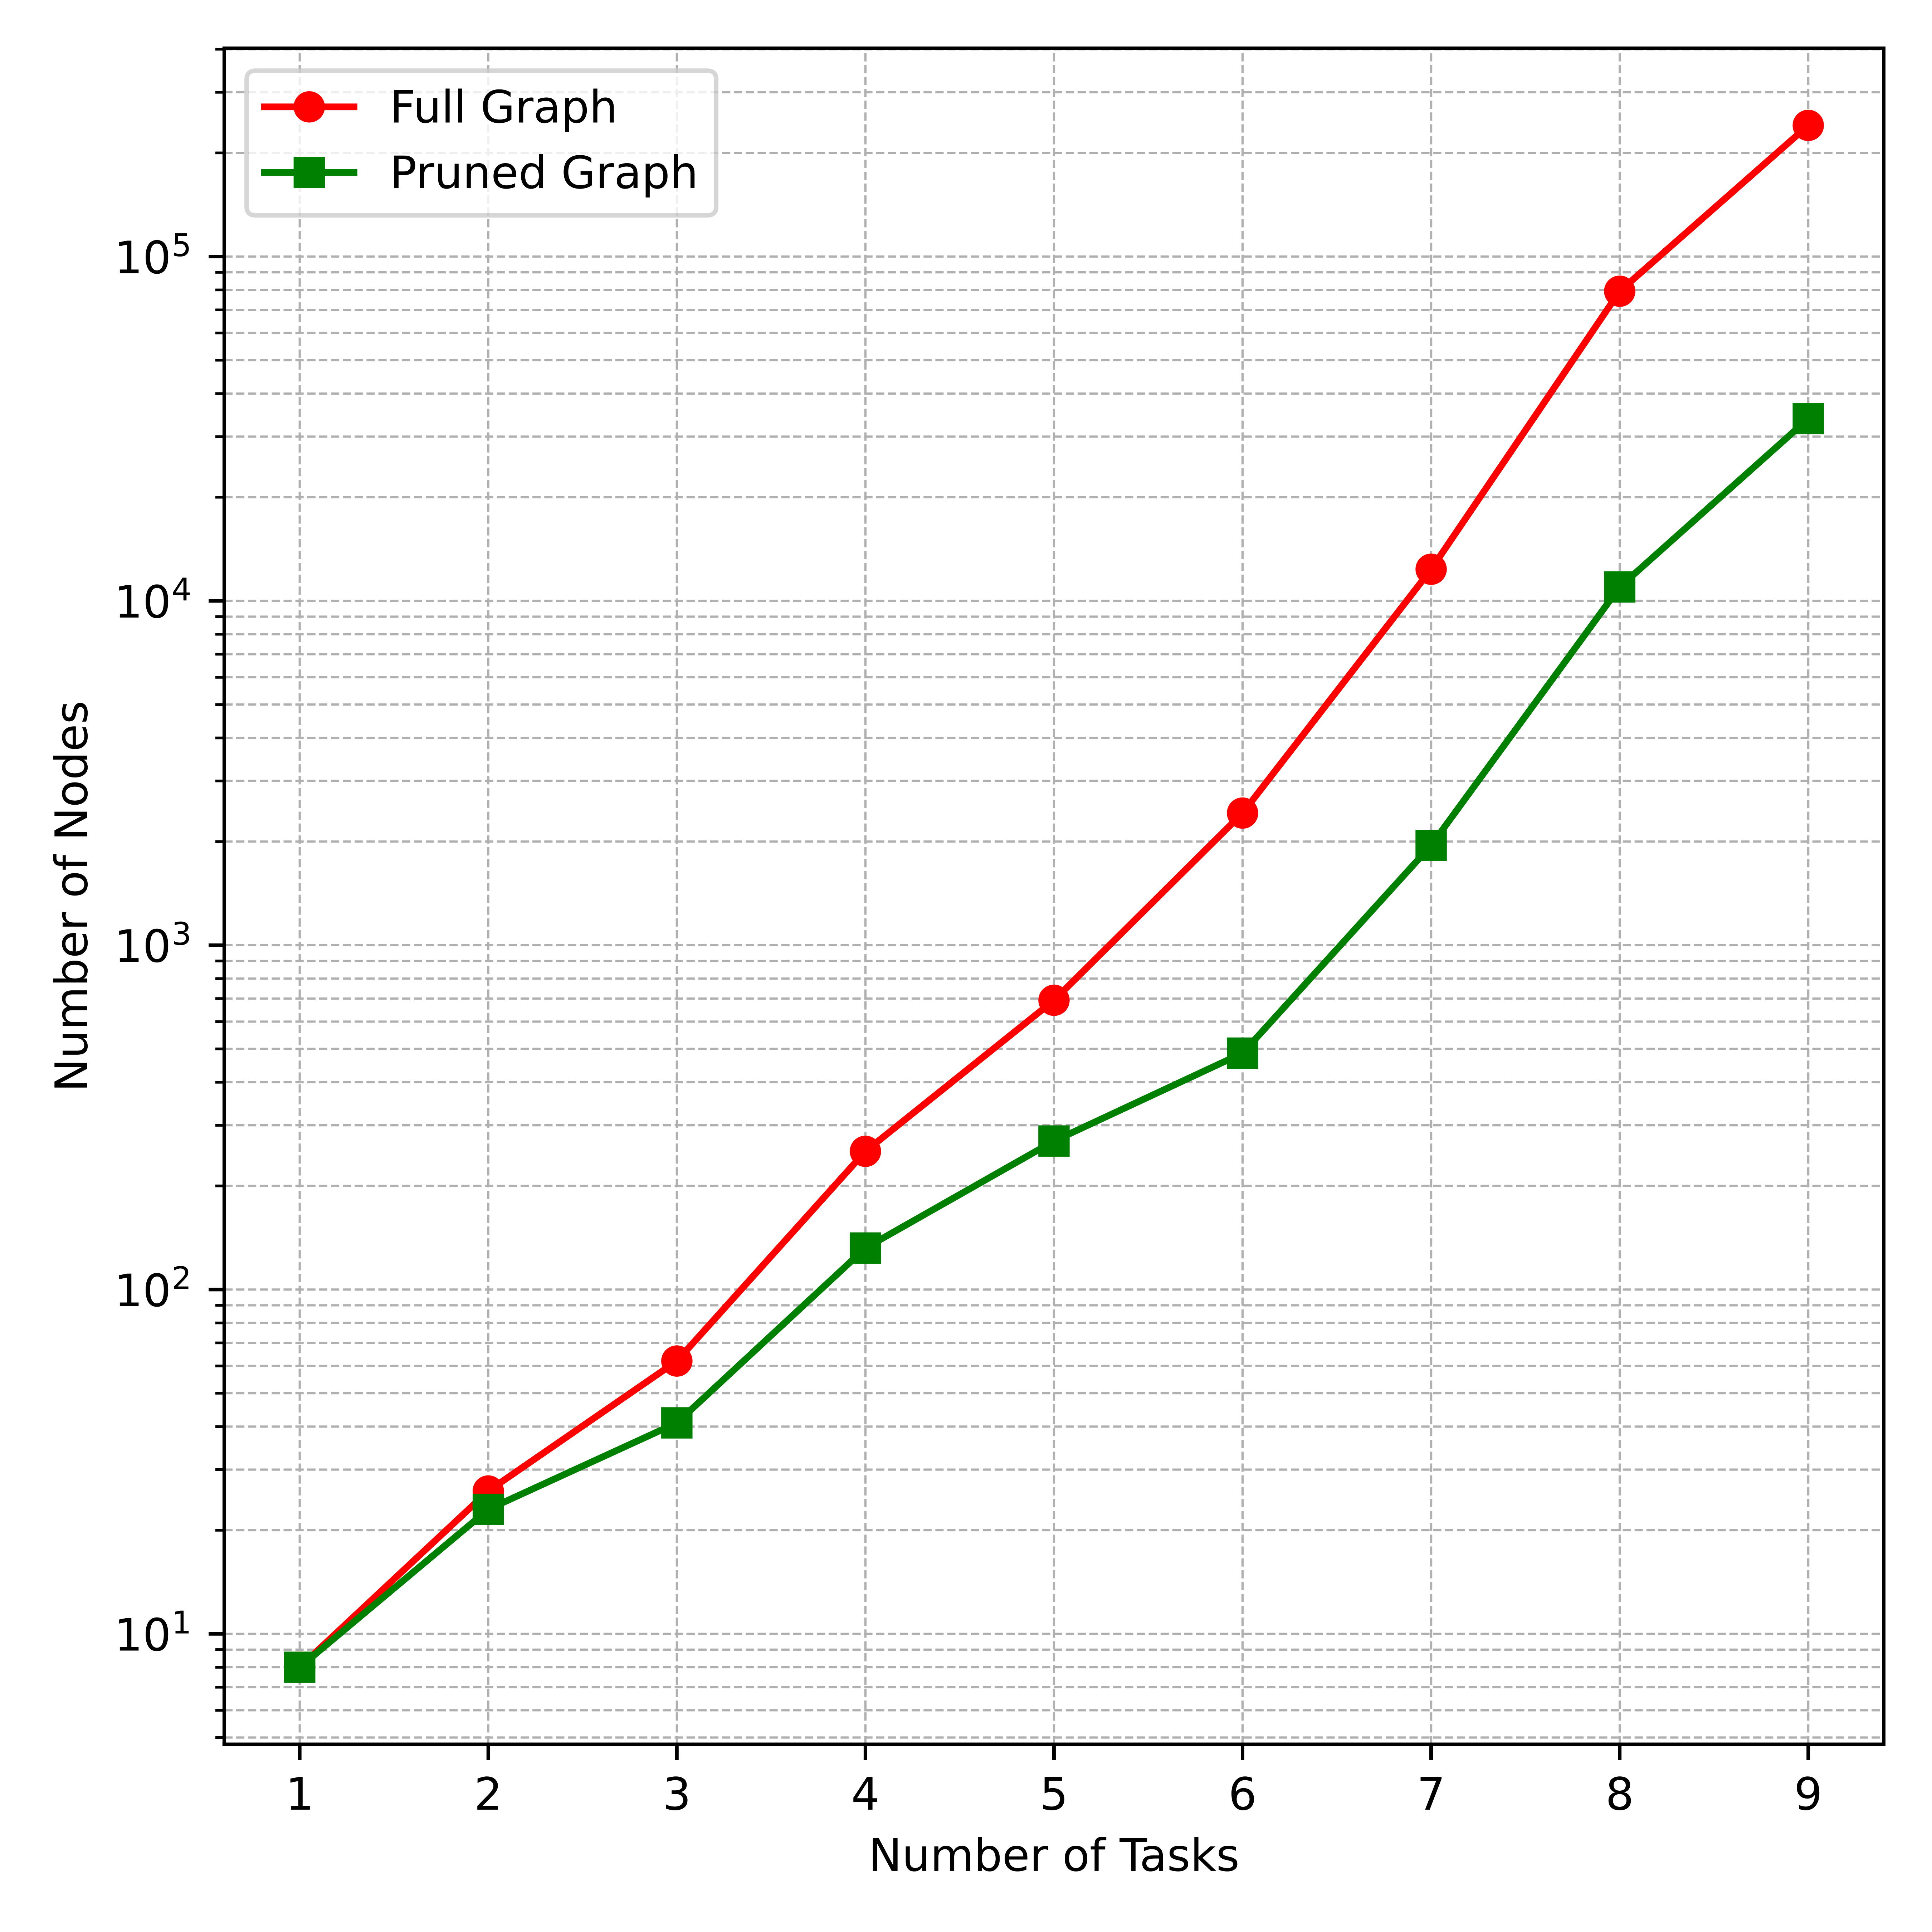
\includegraphics[width=.45\linewidth]{gfx/ch03/gs_graph_size_plot.png}} \quad
    \subfloat[Processing time vs. number of weeds]
    {\label{fig:graphsearch-processing-time}%
        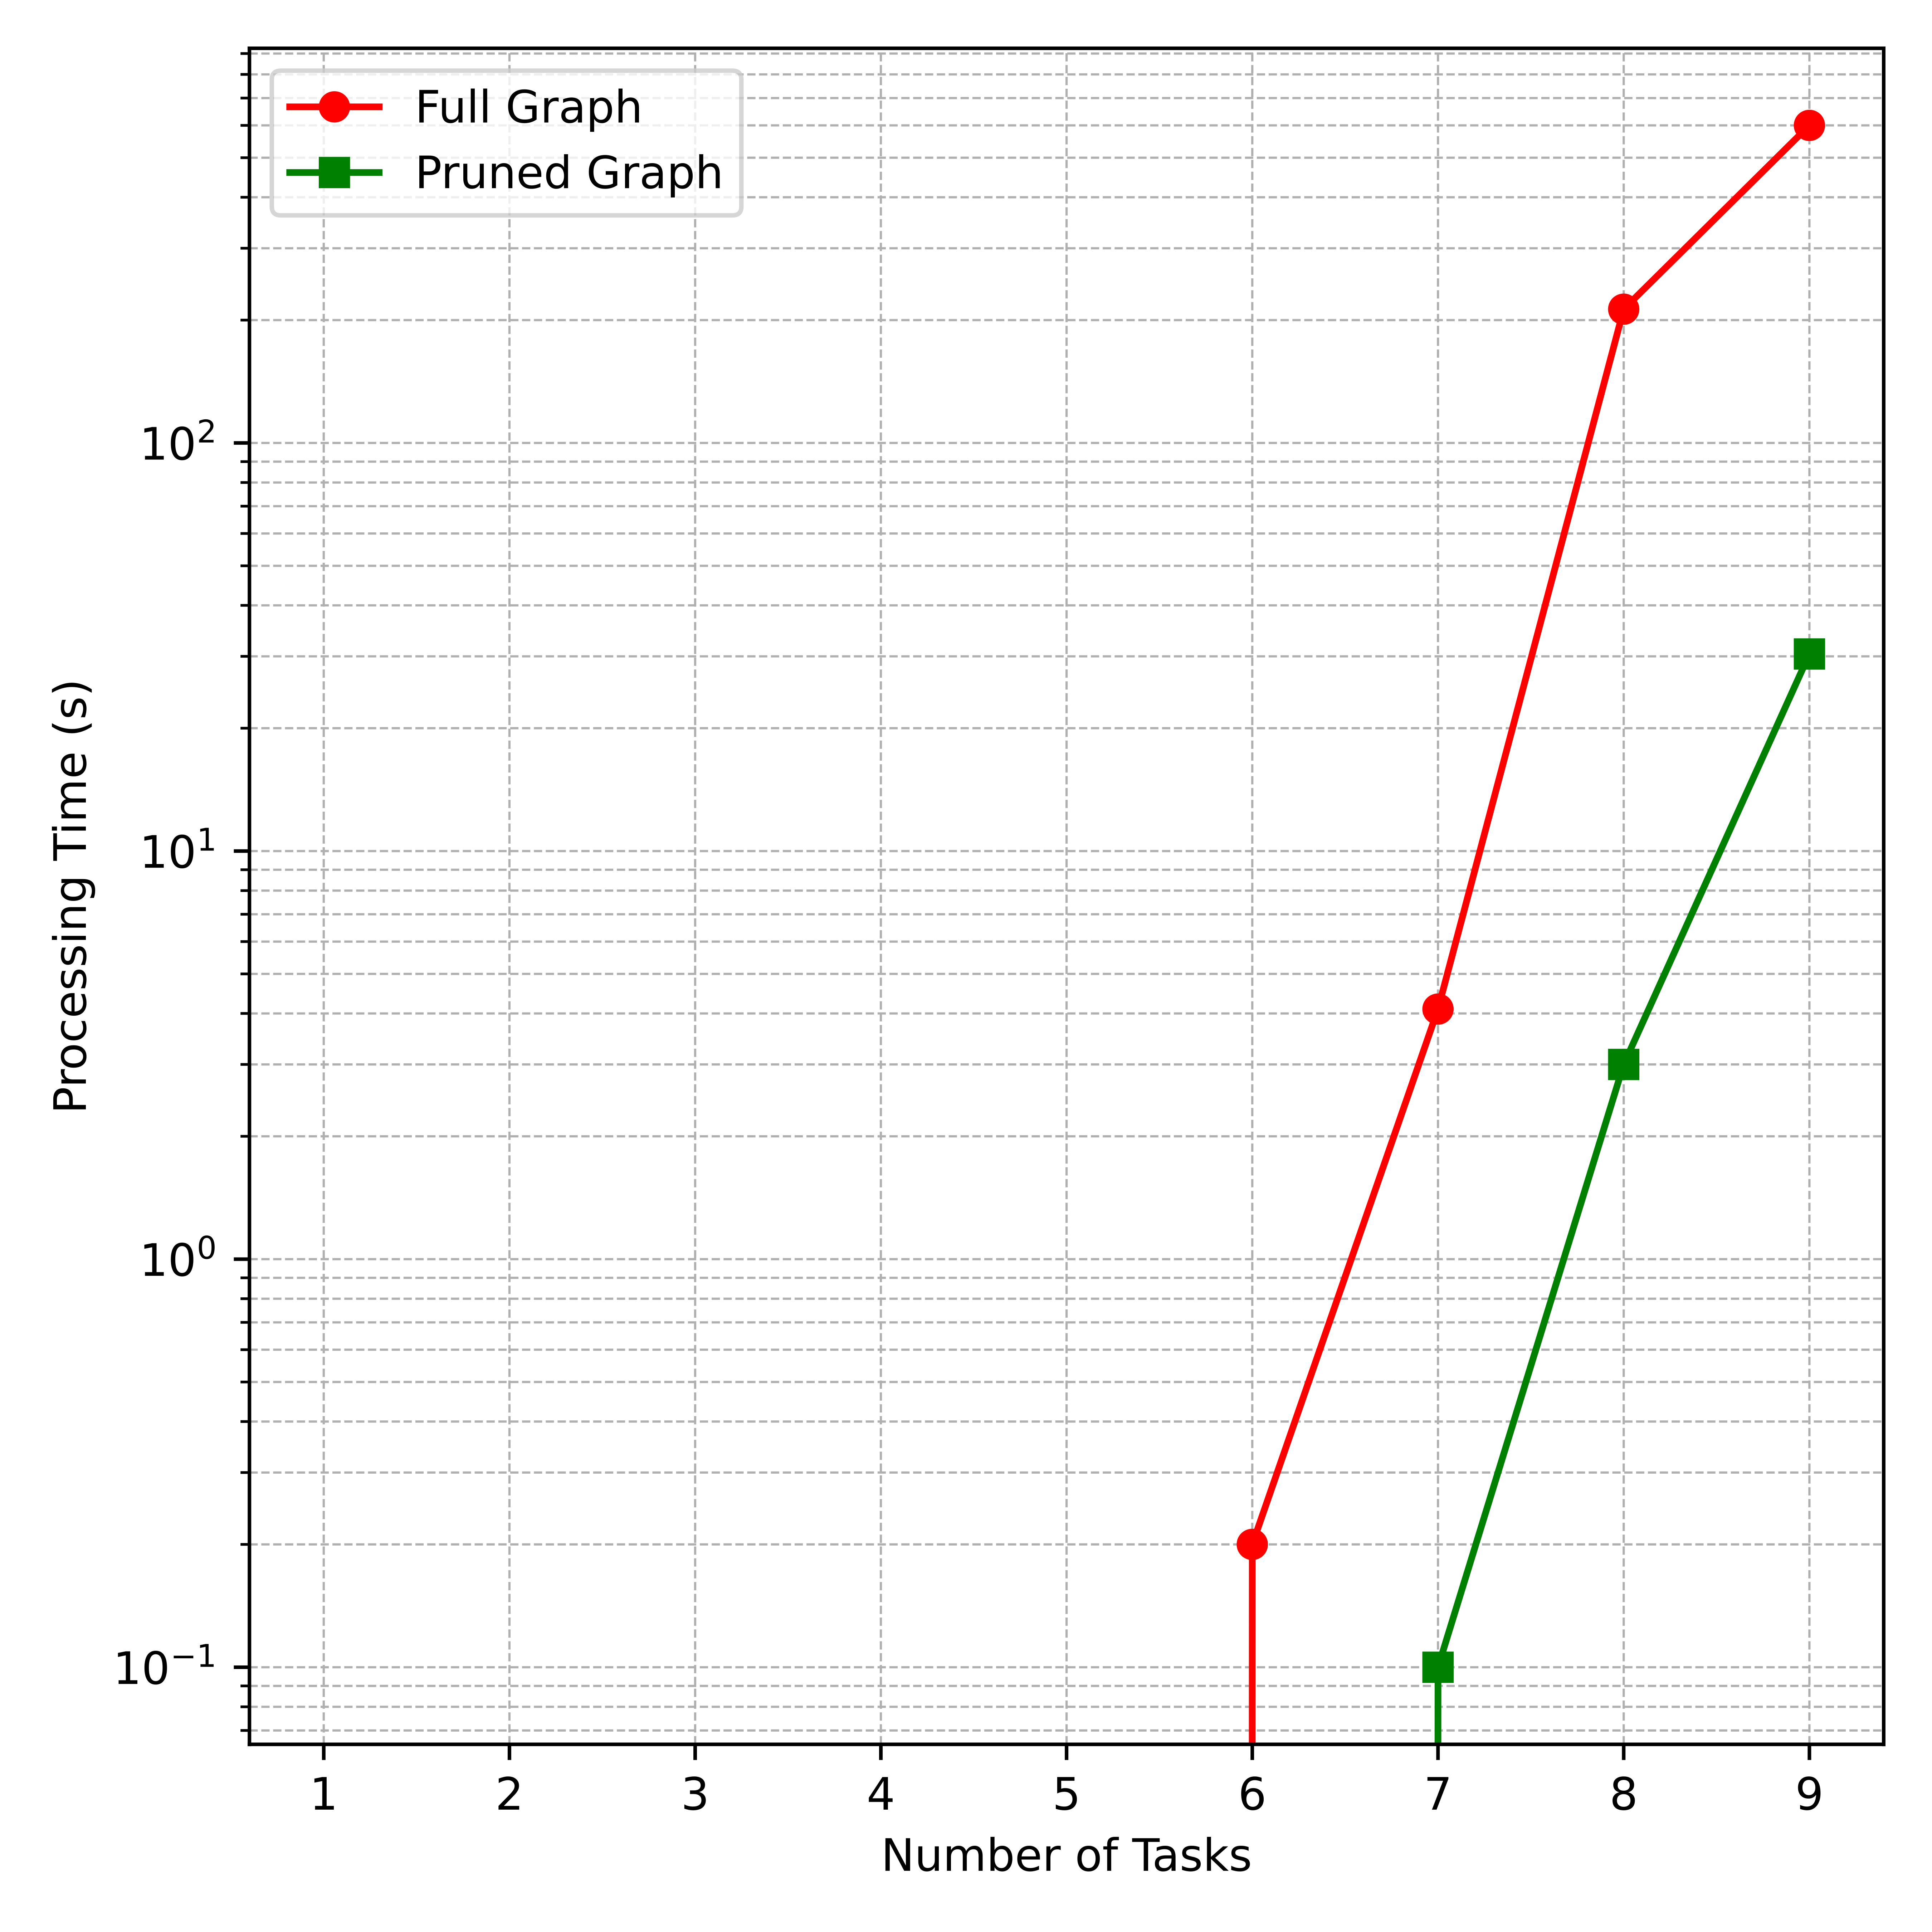
\includegraphics[width=.45\linewidth]{gfx/ch03/gs_proce_time_plot.png}} \\
    \caption{Graph Search algorithm performance}\label{fig:graphsearch-performance}
\end{figure}

We were able to optimize and reduce the graph size by applying a pruning technique that stops the growth of certain branches when they are not promising. This is achieved by introducing the concept of \textit{expired tasks}, these are tasks that haven't been removed and can no longer be removed in future stops because the corresponding weeds have been left behind, outside the tool's workspaces. This pruning is implemented in the \texttt{get\_children\_nodes} method, where each task is checked for expiration before being added to the graph. As a result, the number of nodes is significantly reduced, improving computation time (observe green plot in \autoref{fig:graphsearch-performance}).

Although the graph search algorithm is a promising approach, it still suffers from the exponential growth of the graph size as the number of weeds increases. This can lead to longer computation times and may not be suitable for real-time applications with high weed densities. In the next section, we will explore optimization-based approaches that can potentially overcome these limitations and provide more efficient solutions.

\section{Optimization}
As discussed at the beginning of this chapter, the main goal of \ac{TA} is to find the best allocation of resources and the optimal sequence of stops while considering the given constraints. Achieving such a solution requires mathematically formulating the scenario as an optimization task, with a clearly defined objective function, set of constraints, and decision variables that fully describe the problem. Optimization-based approaches are powerful tools that provide a systematic way to find the best feasible solution to a problem by exproring the solution space. Depending on the nature of the problem, a different optimization formulation can be used, such as linear programming, \ac{MIP}, or nonlinear programming. In our case, we will focus on \ac{MIP} as the most suitable approach for the problem.

\ac{MIP} is a mathematical optimization technique that combines both integer and continuous variables in the formulation of the problem. It allows for the modeling of complex decision-making scenarios where some variables must take on discrete values (e.g., binary decisions) while others can take on continuous values. This flexibility makes \ac{MIP} particularly useful for problems that involve resource allocation, scheduling, and other combinatorial optimization tasks. \\

Given a set of tasks $\mathcal{T} = \{1,2,...,T\}$ where each task $j \in \mathcal{T}$ corresponds to one weed detection from a total $T$, and a set of candidate stops $\mathcal{S} = \{1,2,...,S\}$ where each stop $i \in \mathcal{S}$ is computed using events as in Graph Search algorithm. Let $x_{i,j} \in \{0,1\} $ be a binary decision variable equal to $1$ if task $j$ is assigned to stop $i$, $0$ otherwise and ${imb}_i \in \mathbb{N}_0$ the imbalance of assigned tasks between tools at stop $i$. We know that from each stop $i$ we can only assign tasks that are visible from that stop, and a subset for those corresponds to tasks set to front or back tools, these statements could be better defined as:

\begin{tabular}{ll}
    $\mathcal{V}_i \subseteq \mathcal{T}$ & Set of tasks visible from stop $i$ \\
    $\mathcal{F}_i \subseteq \mathcal{V}_i$ & Front tool task assigned at stop $i$ \\
    $\mathcal{B}_i \subseteq \mathcal{V}_i$ & Back tool task assigned at stop $i$ \\
    $\tau$ & Constant processing time per task \\
\end{tabular}

We know that each task must be assigned to exactly one stop.

\begin{equation}
    \sum_{i=1}^{S} x_{i,j} = 1 \quad \forall j \in \mathcal{T}
\end{equation}

While visible tasks can only be assigned its corresponding stops.

\begin{equation}
    x_{i,j} = 0 \quad \text{if} \quad j \notin \mathcal{V}_i
\end{equation}

The imbalance per stop is the absolute time difference between front and back tools.

\begin{equation}
    f_i = \sum_{j \in \mathcal{F}_i} x_{i,j} \quad \text{and} \quad b_i = \sum_{j \in \mathcal{B}_i} x_{i,j}
\end{equation}

We want the imbalance ${imb}_i$ to reflect the time difference between front and back processing times at each stop. Therefore, we define the imbalance as the maximum of the two possible differences.

\begin{equation}
    \left| \tau (f_i - b_i) \right| = \max \left( f_i - b_i, b_i - f_i \right)
\end{equation}

Thus

\begin{equation}
    {imb}_i \geq \tau \left(f_i - b_i\right) \quad \text{and} \quad {imb}_i \geq \tau \left(b_i - f_i\right)
\end{equation}

Or equivalently

\begin{equation}
    {imb}_i \geq \left| \tau (f_i - b_i) \right| \quad \forall i \in \mathcal{S}
\end{equation}

The objective function is to minimize the total idle time, expressed as follows

\begin{equation}
    \min \sum_{i=1}^{S} {imb}_i
\end{equation}

Given the constraints and objective function, we can formulate the optimization problem as follows:

\begin{equation}
    \begin{aligned}
        \text{minimize} & \quad \sum_{i=1}^{S} {imb}_i \\
        \text{subject to} & \quad \sum_{i=1}^{S} x_{i,j} = 1 \quad \forall j \in \mathcal{T} \\
                          & \quad x_{i,j} = 0 \quad \text{if} \quad j \notin \mathcal{V}_i
    \end{aligned}
\end{equation}

An advantage of an optimization-based approach is that once the problem is formulated we can use existing optimization libraries to obtain the solution. In our case, we used the \texttt{Google OR-Tools}\footnote{OR-Tools is an open source software suite for optimization, tuned for tackling the world's toughest problems in vehicle routing, flows, integer, linear, and constraint programming. \url{https://developers.google.com/optimization}} library to solve our combinatorial problem.

The pipeline for the optimization-based approach is as follows:
\begin{enumerate}
    \item Compute \textbf{candidate stops} based on the robot's current position and weed detections.
    \item \textbf{Associate} reachable weeds with candidate stops.
    \item Build the \textbf{optimization model} using decision variables, constraints, and objective function.
    \item \textbf{Call solver} to get solution.
    \item \textbf{Decode solution} and return the next optimal stop and task allocation as the algorithm's output.
\end{enumerate}

This method does not suffer from high processing times as weed density increases. The algorithm consistently returns a solution in less than 0.1 seconds across a range of weed densities, from low to extremely high (tested up to $6.25$ weeds/m²), making it a strong candidate for real-time applications. The optimization model effectively balances tasks between tools while minimizing idle time. \autoref{fig:mip-solution} illustrates an example of the solution generated by the optimization algorithm in a scenario with twenty weeds.

\begin{figure}[htb]
    \myfloatalign
    \subfloat[Optimization Output]
    {\label{fig:mip-algorithm-output}
        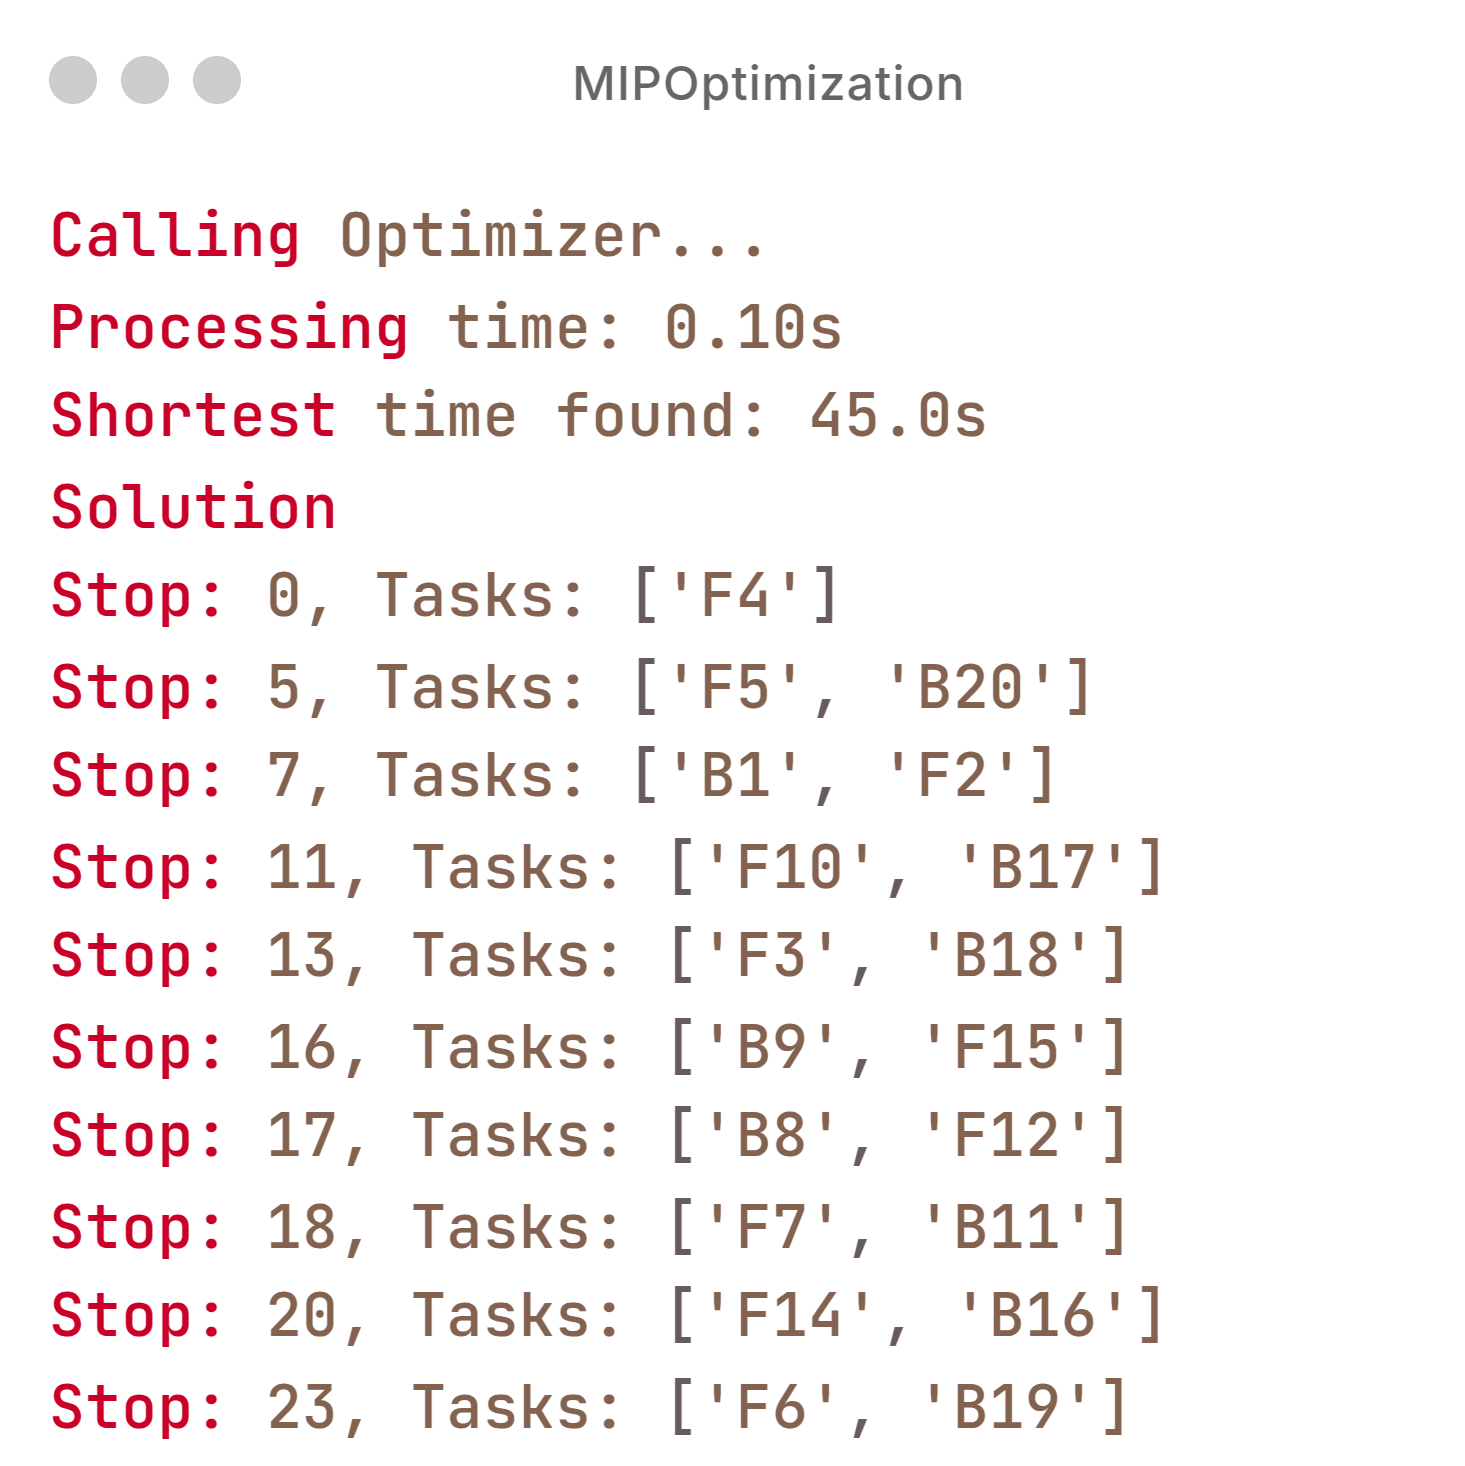
\includegraphics[width=.40\linewidth]{gfx/ch03/mip_solution.png}} \quad
    \subfloat[Task Planning Visualization]
    {\label{fig:mip-scenario-10-tasks}%
        \includegraphics[width=.55\linewidth]{gfx/ch03/mip_scenario_20tasks.png}} \\
    \caption{Mixed-Integer Programming Solution}\label{fig:mip-solution}
\end{figure}

\section{Market-based}
Market-based approaches are a class of algorithms that leverage the principles of supply and demand to solve task allocation problems. In our context, we consider the set of visible tasks from each candidate stop ($\mathcal{V}_i \subseteq \mathcal{T}$). Given these tasks, the algorithm forms all possible combinations of allocations and generates a bid for each one. The allocation is then determined based on the bids received and selecting the best one. A '\textit{better bid}' is defined as the combination that maximizes the number of removed weeds while minimizing the imbalance between tools (i.e., idle time). The algorithm is designed to be fast and efficient, making it suitable for real-time applications. Nevertheless, since the approach always selects the best next stop, it falls into the category of greedy algorithms due to its shortsighted nature. In some cases, it is necessary to sacrifice productivity at the next stop to benefit the overall solution, as illustrated in \autoref{fig:heuristics-suboptimal} and \autoref{fig:heuristics-optimal}. The main advantage of this approach is its ability to adapt to dynamic environments where tasks change over time.

The next stop computation follows a similar pipeline to previous algorithms, with the main differences being the use of a bidding process to determine the best solution and the computation of candidate stops. Algorithm~\ref{alg:run-algorithm} outlines the steps involved during the algorithm.

\begin{algorithm}
    \caption{Run Algorithm (Market-Based)}
    \label{alg:run-algorithm}
    \begin{algorithmic}[1]
    \REQUIRE Current tasks and robot pose
    \ENSURE Best stop and task assignment with shortest idle time
    
    \STATE $\texttt{candidate\_stops} \gets \texttt{get\_candidate\_stops()}$
    \STATE \texttt{associate\_tasks\_with\_stops(candidate\_stops)}
    \IF{\texttt{log\_print}}
        \STATE \texttt{log("Collecting Biddings...")}
    \ENDIF
    \STATE \texttt{start\_timer()}
    \STATE $(\texttt{stop}, \texttt{tasks}, \texttt{idle\_time}) \gets \texttt{get\_best\_bid()}$
    \STATE $\texttt{sw\_time} \gets \texttt{stop\_timer()}$
    \IF{\texttt{log\_print}}
        \STATE \texttt{log("Processing time: "} $\texttt{sw\_time}$\texttt{"s")}
        \STATE \texttt{log("Shortest time found: "} $\texttt{idle\_time}$\texttt{"s")}
    \ENDIF
    \STATE \textbf{return} $(\texttt{stop}, \texttt{tasks}, \texttt{idle\_time})$
    \end{algorithmic}
\end{algorithm}
    
The candidate stops are computed by considering only the closest weed detection and the events this task generate within the back tool workspace. These events include:

\begin{enumerate}
    \item Entering the workspace.
    \item The stop position where the weed is about to exit (rather than when it fully exits).
\end{enumerate}

Using these two candidate poses, we generate evenly distributed positions to create additional candidates between these two events. Afterwards, we perform task association per stop as usual and call \texttt{get\_best\_bid} to start the bidding process and obtain the solution. The algorithm iterates through all possible combinations of tasks at each stop, calculating the idle time for each combination. The combination with the lowest idle time and more number of weeds is selected as the best bid. This process is repeated for all candidate stops, and the best overall stop and task allocation are returned (observe Algorithm \ref{alg:get-best-bid}).

\begin{algorithm}[H]
    \caption{Get Best Bid}
    \label{alg:get-best-bid}
    \begin{algorithmic}[1]
    \REQUIRE Candidate stops with associated tasks
    \ENSURE Best stop and task assignment with minimum idle time
    
    \STATE $\text{bid} \gets \text{Bid}(\emptyset, \infty)$
    \STATE $\text{stops} \gets [\ ]$
    \STATE $\text{best\_stop} \gets \text{None}$
    \STATE $\text{best\_bid} \gets \text{None}$
    
    \FOR{$i, \text{stop} \in \text{enumerate(candidate\_stops)}$}
        \STATE $\text{tasks\_per\_stop} \gets [\ ]$
        \FOR{$\text{task} \in \text{stop["tasks"]}$}
            \STATE $\text{tasks\_per\_stop.append(task)}$
        \ENDFOR
    
        \STATE $\text{combinations} \gets \text{get\_all\_combinations(tasks\_per\_stop)}$
        \STATE $\text{idle} \gets \text{get\_idle\_per\_combination(combinations)}$
        \STATE $\text{bid} \gets \text{get\_bid(zip(combinations, idle))}$
        \IF{\text{update\_bid\_if\_better(bid)}}
            \STATE $\text{best\_stop} \gets i$
            \STATE $\text{best\_bid} \gets \text{bid}$
        \ENDIF
    \ENDFOR
    
    \RETURN $\text{stops[best\_stop]}, \text{best\_bid.tasks}, \text{best\_bid.idle}$
    \end{algorithmic}
\end{algorithm}
    

An example of the solution produced by this algorithm is illustrated in \autoref{fig:mkt-solution}. We can observe that only four candidate stops are generated for four tasks. Notice the contrast with the graph search in \autoref{fig:scenario-2-tasks} and the optimization approach in \autoref{fig:mip-scenario-10-tasks}.

\begin{figure}[htb]
    \myfloatalign
    \subfloat[Market-based Output]
    {\label{fig:mkt-algorithm-output}
        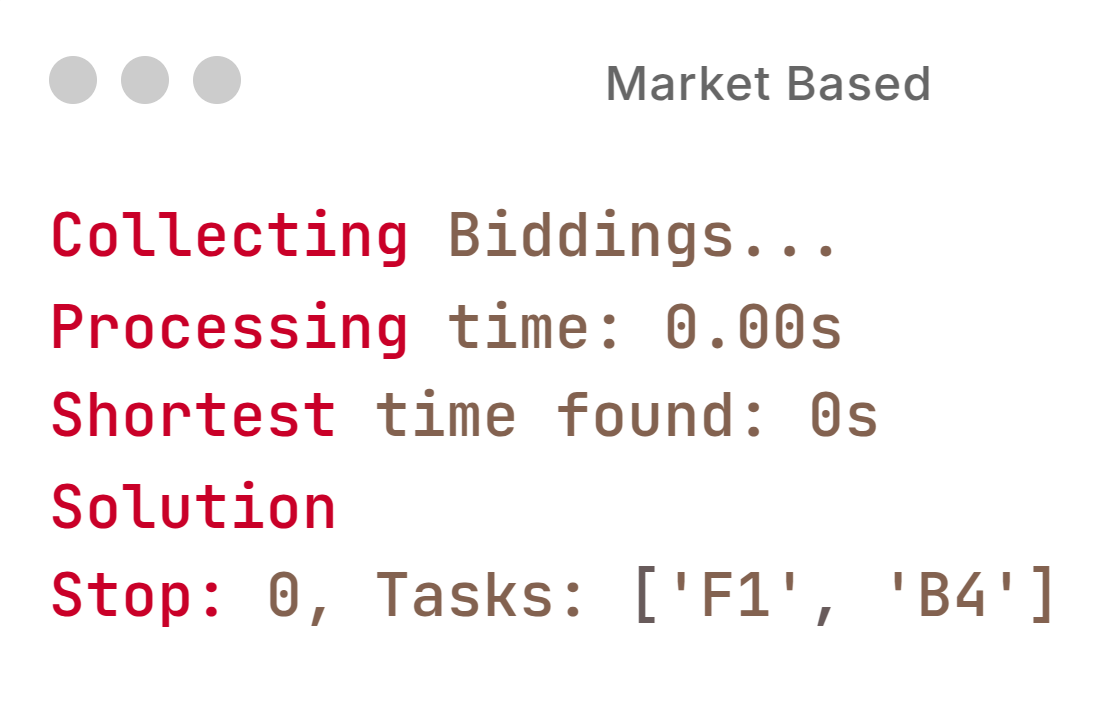
\includegraphics[width=.45\linewidth]{gfx/ch03/mkt_solution.png}} \quad
    \subfloat[Task Planning Visualization]
    {\label{fig:mkt-scenario-4-tasks}%
        \includegraphics[width=.50\linewidth]{gfx/ch03/mrk_scenario_4tasks.png}} \\
    \caption{Market-based Solution}\label{fig:mkt-solution}
\end{figure}

%*****************************************
%*****************************************
%*****************************************
%*****************************************
%*****************************************
